%%%% University of Cambridge tech-report formatting; enable when producing
%%%% tech-report versions of these documents; otherwise, disable.
%\documentclass[12pt,twoside,openright,a4paper]{report}
%\setlength{\oddsidemargin}{-0.4mm} % 25 mm left margin
%\setlength{\evensidemargin}{\oddsidemargin}
%\setlength{\textwidth}{160mm}      % 25 mm right margin
%\setlength{\topmargin}{-5.4mm}     % 20 mm top margin
%\setlength{\headheight}{5mm}
%\setlength{\headsep}{5mm}
%\setlength{\footskip}{10mm}
%\setlength{\textheight}{237mm}     % 20 mm bottom margin
%%%% .. or regular document
\documentclass[12pt,letterpaper,twoside,openright,fleqn]{report}
%%%% End of tech-report vs. regular
%%%%

%\renewcommand{\baselinestretch}{2} % double space for editors 
\usepackage{fullpage}
\usepackage{graphicx}
\usepackage{marginnote}
\usepackage{appendix}
\usepackage{booktabs}
\usepackage{bytefield}
\usepackage{color}
\definecolor{lightgray}{gray}{0.8}
\usepackage{times}
\usepackage{algpseudocode}
\newcommand{\note}[2]{{\color{blue}[ Note: #1 - #2]}}
\usepackage{listings}
\usepackage{setspace}
\usepackage{amsmath}
\usepackage[nounderscore]{syntax}
% Must be included later than setspace, otherwise all footnote hyperlinks
% point to the title page.
\usepackage{hyperref}
\definecolor{CodeColour}{rgb}{0.9,0.9,0.9} %Light grey
\lstset{basicstyle=\small\ttfamily,
        stringstyle=\textit, %italic strings
        keywordstyle=\color{red}\textbf, %Bold keywords
        commentstyle=\color{blue},
        breaklines=true, % Wrap long lines
        numbers=left, % Line numbers on the left
        frame=l, %Border on the left
        framerule=0.8pt, % Thick border
        backgroundcolor=\color{CodeColour}, %Coloured code listings
        numberstyle={\small \oldstylenums},  %tiny, old style line numbers
		%stepnumber=5, % Number every fifth line
        numbersep=5pt, % Five points between the line numbers and the text
        tabsize=4
}
\lstdefinelanguage{llvm}
{
	morekeywords={private, constant, i8, i32, define, icmp, label, i64, call, void, ret, getelementptr, br, load, align, nounwind},
	morekeywords={addrspace, inttoptr, ptrtoint, tail},
	morecomment=[l];
}%

\lstnewenvironment{ccodelisting}{\lstset{language=C}}{}
\lstnewenvironment{llvmlisting}{\lstset{language={llvm}}}{}
\newcommand{\ccode}[1]{\lstinline[backgroundcolor=\color{white},language=C]|#1|}
\newcommand{\llvmir}[1]{\lstinline[backgroundcolor=\color{white},language={llvm}]|#1|}
\newcommand{\asm}[1]{\lstinline[backgroundcolor=\color{white},language={}]|#1|}
\lstnewenvironment{asmcode}{\lstset{language=}}{}
\newcommand{\regname}[1]{{\small\ttfamily\$#1}}

\hyphenation{CADETS}

\reversemarginpar
\setlength{\marginparwidth}{1.2in}
\let\oldmarginpar\marginpar
\renewcommand\marginpar[1]{\-\oldmarginpar[\raggedright\footnotesize #1]%
{\raggedright\footnotesize #1}}

\newcommand{\pathname}[1]{{\texttt{\detokenize{#1}}}}
\newcommand{\literal}[1]{{\texttt{\detokenize{#1}}}}
\newcommand{\function}[1]{{\texttt{\detokenize{#1}}}}
\newcommand{\instruction}[1]{{\texttt{#1}}}
\newcommand{\register}[1]{{\texttt{\%#1}}}
\newcommand{\registerop}[1]{{\texttt{\textbf{#1}}}}
\newcommand{\nregs}{{\texttt{\textbf{NREGS}}}}
\newcommand{\subroutine}[1]{{\texttt{\detokenize{#1}}}}
\newcommand{\struct}[1]{{\texttt{\detokenize{#1}}}}


\begin{document}
\title{OpenDTrace Object Format (DOF) and \\
  OpenDTrace Intermediate Format (DIF) \\
  Specification \\
  {\large Version 0.1 - DRAFT}
}

\date{August 16, 2017}

\author{
  Robert N. M. Watson, George Neville-Neil, and Domagoj Stolfa \\
  \\
  BAE Systems, The University of Cambridge, \\
    and Memorial University Newfoundland
}

%% CL tech-report format provides its own cover page
\begin{minipage}[h]{\textwidth}
  \maketitle

  \vspace{2in}
  {\small
  Approved for public release; distribution is unlimited.
  Sponsored by the Defense Advanced Research Projects Agency (DARPA) and the
  Air Force Research Laboratory (AFRL), under contracts FA8650-15-C-7558
  (``CADETS'') as part of the DARPA Transparent Computing research program.
  The views, opinions, and/or findings contained in this report are those of the
  authors and should not be interpreted as representing the official views or
  policies, either expressed or implied, of the Department of Defense
  or the U.S. Government.}
\end{minipage}
%%

\normalsize

%% CL tech-report format requires page numbering to start at 3
%\setcounter{page}{3}
%%

%% For revisions sent for editing, prefer double spacing.
%\doublespacing
%%

\clearpage

\section*{Abstract}

DTrace is a dynamic tracing facility offering full-system instrumentation, a
high degree of flexibility, and portable semantics across a range of
operating systems.
Originally designed and implemented by Sun Microsystems (now Oracle),
user-facing aspects of DTrace, such as the D language and command-line tools,
are well defined and documented.
However, DTrace's internal formats -- the DTrace Intermediate Format (DIF) and
DTrace Object Format (DOF) -- have primarily been documented through source
code comments rather than a structured specification.
This technical report specifies these formats in order to better support the
development of more comprehensive tests, new underlying execution subtrates
(such as just-in-time compilation), and future extensions.
%DIF is a RISC bytecode into which D scripts are compiled, describing the
%specific executable actions in a script.
%DOF is the container format containing a set of headers and sections for
%variables, probe implementations, constants, and other content required to
%represent a complete script.


\clearpage

\section*{Acknowledgments}
The authors of this report thank the creators of DTrace, including
Bryan Cantril, Adam Leventhal and Michael Shapiro for a spectacular
contribution to the field of operating-system design, and in
particular for designing the data structures, instructions, and other
elements of DTrace described in this specificaiton.  Some of the text
in this specification has been excerpted from the excellent comments
present in the original source code.

One cannot work with DTrace without running across the work of Brendan
Gregg, author of the DTrace Toolkit, as well as \emph{DTrace: Dynamic
  Tracing in Oracle Solaris, macOS and FreeBSD}, and to him we also
owe a debt of thanks.

Several people, including some of the original developers of DTrace,
reviewed this report during various stages of its development and so
we'd like to extend our thanks to Matthew Ahrens, Mark Johnston,
Samuel Lepetit, Adam Leventhal, and David Pacheco.

The authors of this report also thank other members of the CADETS team, and
our past and current research collaborators at BAE Systems, the University of
Cambridge, and Memorial University Newfoundland:

%
% Various folk including interns and co-authors on papers supported in part by
% CADETS.
%
\begin{tabular}{llll}
  Jon Anderson & David Chisnall & Silviu Chiricescu & Brooks Davis \\
  Khilan Gudka & Ben Laurie & Ilias Marinos & Peter G. Neumann \\
  Greg Sullivan & Rip Sohan & Amanda Strnad & Bjoern Zeeb
\end{tabular}

\bigskip

%\noindent
%The CADETS team also thanks past and current members of its external
%oversight group for significant support and contributions:
%
%\bigskip
%
%\begin{tabular}{llll}
%\end{tabular}
%
%\bigskip

The port of DTrace to FreeBSD was carried out in 2007 by John Birrell
who, sadly, passed away in 2009, and we dedicate this report to his
memory.

\noindent
Finally, we are grateful to Angelos Keromytis, DARPA Transparent Computing
program manager, who has offered both technical insight and support throughout
this work.


\clearpage

\tableofcontents

\clearpage

\chapter{Introduction}
\label{chap:introduction}
OpenDTrace is a dynamic tracing facility integrated into the Solaris,
FreeBSD, and macOS operating systems\textemdash with ports also available for
Linux and Windows.  Dynamic tracing allows system administrators and
software developers to develop short scripts (in the D programming
language) that instruct OpenDTrace to instrument aspects of system
operation, gather data, and present it for human interpretation or
mechanical processing.  While there is excellent documentation
available for the D programming language, command-line tools, and
OpenDTrace-based investigation and operation, the internal formats to
OpenDTrace are generally documented via the source code.  This report
acts as a \textit{de facto} specification for those formats, including the
DTrace Intermediate Format (DIF), which is a bytecode that D scripts
are compiled into for safe execution within the kernel, and the DTrace
Object Format (DOF), which bundles together complete scripts along
with their associated constants and metadata.

%\section{Motivation}
\section{Background}

The original DTrace code was designed and developed by Sun
Microsystems to solve a particular problem, being able to instrument
systems that were currently deployed, without requiring the
recompilation of any code \cite{DTrace2004}.  The DTrace system was
written in a portable style typical of code from the Sun Microsystems
Kernel Development group in the early 2000s.  Shortly after the
release of the original DTrace system a port was made, by John Birrel,
to the FreeBSD Operating System.  A port was also made by Apple to
their macOS at about the same time.  DTrace gained popularity as a
dynamic tracing system throughout the first decade of the 21st Century
and its usage is well documented
\cite{mckusick2014design}\cite{Microsystems2008a}\cite{Gregg:2011:DDT:1971960}.

The OpenDTrace system is meant to capture information about systems at
run time, without the need to stop the program or kernel being
investigated.
A tracing system captures the program state of a running program and
can show changes in that state over time.  The person who is
initiating the trace must decide before starting what information they
wish to capture.  Tracing systems have an important design constraint,
which is the need to make the tracing system itself have as low an
impact on overall system performance as possible.

From the perspective of the user the OpenDTrace model is one of
\emph{Plan}, \emph{Capture} and \emph{Analyze}.  The \emph{Plan} phase
is where the user writes brief scripts, in the D langauge, that
describe the probe points from which they wish to capture data.
Conditions can be placed upon when these probe points are active, so
that the amount of data captured in the next phase, can be narrowed
down to only what is absolutely neessary to feed the analysis and
answer the question we are asking of the system.  The \emph{Capture}
phase is triggered by the \texttt{dtrace} program pushing the plan,
in the form of compiled code, into the operating system's kernel which
activates the required probe points.  The OS kernel captures the data
into bufers which are eventually fed out to user space, where they can
be analyzed.  The \emph{Analysis} is undertaken in user space where
the previously written plan, in the form of D scripts, directs the
OpenDTrace library to extract, display and or aggregate the captured
data.  Many workflows currently require some form of post-processing
of the data captured for analysis, and this post-processing is
currently carried out on unstructured text.

OpenDTrace is made up of several components, including kernel code,
user space libraries, and command line tools.  The OpenDTrace system
uses information generated during code compilation to expose a set of
trace points with which users and programs can interact.  These trace
points can be the entry and exit points of functions as well as system
calls, or they can be arbitrary points in the instruction stream,
marked out with a set of standardized macros.  From the user's point
of view tracing is activated by a command line program,
\texttt{dtrace}, but any program that is compiled with the OpenDTrace
libraries may initiate tracing, so long as it has sufficient
privileges.

The OpenDTrace privilege model is relatively simple, any program that
wishes to trace another program must be running with \emph{root}
privileges.  Some operating systems, such as Illumos, provide a more
nuanced privilege model, the details of which are discussed further in
Section~\ref{sec:privilege}.

Tracepoints are collected into one of many \emph{providers} which dictate
the capabilites of the tracepoint and how it interacts with the overall
tracing system.  Providers exist for system calls (\texttt{syscall}),
function boundary tracing (\texttt{fbt}), timing services (\texttt{profile}),
as well as specific subsystems such as the network (\texttt{ip}, \texttt{tcp}),
filesystem (\texttt{vfs}) and process scheduler (\texttt{proc}).
Arbitrary trace points can be added to the kernel via the
statically defined trace point (\texttt{sdt}) provider.  User space programs
are traced either with the \texttt{pid} provider or using the 
statically defined trace point (\texttt{usdt}) provider.  

% A complete list of providers is given in Appendix~\ref{chap:opendtrace-providers}.

\section{The OpenDTrace Project}
\label{sec:opendtrace-project}

The OpenDTrace project exists to be a single, cross platform, upstream
source of tracing code.  Based initially on the DTrace code that was
written by Sun Microsystems, now Oracle, for the OpenSolaris and then
Illumos operating system the code has already been ported to FreeBSD,
by Jon Birrell, and macOS, by engineers working internally at Apple
Computer.  OpenDTrace combines all of these divergent ports into a
single source tree that can be deployed on any of these three
operating systems, with a unified set of features.  

The OpenDTrace project maintains its own organization on github
(https://github.com/opendtrace) with a set of repositories, including
one for documentation (https://github.com/opendtrace/documentation)
from whence this specification originates.

THe OpenDTrace team welcome contributions of code, bug fixes, and
other information via pull requests to the relevant repositories
within the github organization.

\section{Version History}

\begin{description}
\item[0.1] This is the first version of the \textit{OpenDTrace Formats
  Specification}, made available for early review and collaborative
  development.
\end{description}

\section{Document Structure}

This report specifies a number of aspects of OpenDTrace's operation:

\begin{description}

\item[The Achitecture of OpenDTrace] described in
  Chapter~\ref{chap:opendtrace-arch} gives a general overview of the
  internals of the OpenDTrace system, including the relationship of
  the major components, privilege model, and other, overarching,
  concerns.

\item[The D Langauge] described in
  Chaper~\ref{chap:opendtrace-dlang} provides a full description of
  the D language, which is the domain specific scripting language used
  to create more complex data queries and to perform data reduction
  after tracepoint data has been captured.

\item[The Compact Trace Format (CTF)] described in
  Chapter~\ref{chap:opendtrace-ctf} explains the data extracted from
  compiled object code that is used by OpenDTrace to create trace
  points and extract function arguments and types.

\item[The OpenDTrace Object Format (DOF)] described in
  Chapter~\ref{chap:opendtrace-object-format} is a file-like format linking
  together a set of sections describing OpenDTrace code, string constants, and
  other aspects of a complete compiled OpenDTrace script.

\item[The OpenDTrace Intermediate Format (DIF)] is the bytecode that the
  executable elements of OpenDTrace scripts are compiled to.
  This is a simple RISC-like instruction set with constrained execution
  properties (e.g., only forward branches).
  Chapter~\ref{chap:opendtrace-intermediate-format} describes the instruction
  format and common instruction semantics.

\item[DTrace Instructions] are the individual RISC instructions
  performing a variety of operations including register access, memory
  access, arithmetic operations, and calling various built-in
  subroutines available to scripts in execution.
  Chapter~\ref{chap:opendtrace-instruction-reference} enumerates the
  instructions, their arguments, and their semantics.

\item[Built-in Global Variables] are a set of implementation-defined
  variables always available to scripts.
  This includes DTrace state (such as the current probe ID) and state from the
  instrumented probe context (e.g., the current process ID).
  Chapter~\ref{chap:opendtrace-global-vars} specifies these variables.

\item[Built-in Subroutines] are available to scripts, providing access to
  higher-level behavior, such as memory copying, string comparison, and so on.
  Chapter~\ref{chap:opendtrace-subroutines} describes the available built-in
  subroutines.

\item[Code Organization] for the DTrace implementation varies by operating
  system.
  Appendix~\ref{chap:opendtrace-code} describes the high-level layout of the
  DTrace code in several operating systems incorporating DTrace support.

%\item[Providers] for OpenDTrace are listed in
%  Appendix~\ref{chap:opendtrace-providers}

\end{description}

\section{Definitions}

In this section, we provide a number of definitions that will be used throughout
the document. We will assume that the reader is familiar with these definitions,
as no definition will be repeated.

\begin{description}
\item[Memory locations] The set of all strictly positive integers.
\item[Memory] An unbounded partial map of memory locations to values at those memory
  locations.
\item[Unpagable memory] An unbounded total map of memory locations to values at those memory
  locations.
\item[D variable memory] A bounded map of strings to values.
\item[Page fault] Attempt to access a memory location in memory which does not map to
  any value, causing a failure.
\item[Paged in memory] In a given memory map, a memory location $\mathcal{l}$ is
  paged in if it exists in the domain of the map.
\item[Allocation] An attempt to create a new relation in a map between memory locations and
  values.
\item[Deallocation] Removing a relation from a map between memory locations and values.
\item[Thread] An execution pattern of a sequence of instructions with a unique identifier.
\end{description}


\chapter{Operational Model}
\label{chap:opendtrace-operation}
The components that make up OpenDTrace interact with each other to
implement an operational model for dynamic tracing.  At the highest
level there are three components to OpenDTrace: tools, such as
\texttt{ctfconvert} which take compiled object code and generate new
ELF/DWARF sections that capture type information, the kernel module,
which is responsible for adding and removing trace points at run time,
and the libraries, which tie all of the components together.  Users
interact with OpenDTrace via the \texttt{dtrace} command line tool.

The OpenDTrace kernel module is the heart of the DTrace
framework. This module is responsible for the coordination of all
other components used in instrumentation. It keeps track of all
registered providers and informs them when to enable or disable their
probes. When a probe fires, the OpenDTrace kernel module is
responsible for executing the necessary instrumentation code and
providing the data to any consumers.

The kernel module is also the intermediary between the DTrace user
interface and the providers. When compiling user scripts, the kernel
module provides the D compiler with probe arguments and types. Once
compiled, scripts are pushed into the kernel as Enabling Code Blocks
(ECBs) to be executed when probes fire. After each ECB is executed,
the data is handed back to user space where the \texttt{dtrace}
command line tool, or other programs linked against the OpenDtrace
libraries can manipulate or display the data to end users.

Providers in OpenDTrace encapsulate the probe points that are used to
instrument code and provide data to the end user. A provider defines
both a set of probe points as well as the standard by which the system
interacts with that set of probe points.  For example the Function
Boundary Tracepoint (fbt) provider defines \texttt{return} trace
points in which only arguments zero ($0$) and one ($1$) are valid and
which always contain the return value and return address
respectively, whereas no other provider has such a definition.

OpenDTrace has a base set of providers that are shipped as part of the
system, see Appendix~\ref{chap:providers}, but developers are free to
create their own, to expose more or different information from their
code. Providers can be developed either for the kernel, in which case
they are defined as kernel modules, or for user space, as part of the
User Defined Static Tracing (USDT) system.

A provider is simply a collection of probe points. Probe points are
functions that are run when certain points in the code are
reached. The probe gathers data of interest and passes data back into
the OpenDTrace kernel module for further processing. Since the
overhead of probes should be avoided when data is not required, the
provider is responsible for tracking when probes are enabled and
implementing a mechanism for the kernel module to update their state.

The user space interface to OpenDTrace is the \texttt{drace(1)}
command line utility, . The \texttt{dtrace} command line utility
handles all run time interaction with the OpenDTrace system, such as
submitting scripts for execution as well as configuring options as
memory usage, and how often the system should flush data from the
kernel.  The complete syntax and set of options for the
\texttt{dtrace} command is given in the manual page.

The majority of the DTrace CLI functionality is provided through calls
to the DTrace user-space library, \texttt{libdtrace}, which is
responsible for setting DTrace options, compiling D scripts, and
passing compiled D code to the kernel for
execution. \texttt{libdtrace} provides the mechanism for all
interactions with DTrace in the kernel.

\section{Probe Life Cycle}
\label{sec:lifecycle}

An example of instrumentation with OpenDTrace is shown in
Figure~\ref{fig:lifecycle}. We assume that the OpenDTrace kernel
module has already been loaded during system boot. We ignore the
execution of code within any of the providers and only discuss the
interactions between components. Internal functions of interest within
the kernel module and CLI are shown.

\begin{figure}[htpb]
	\centering
	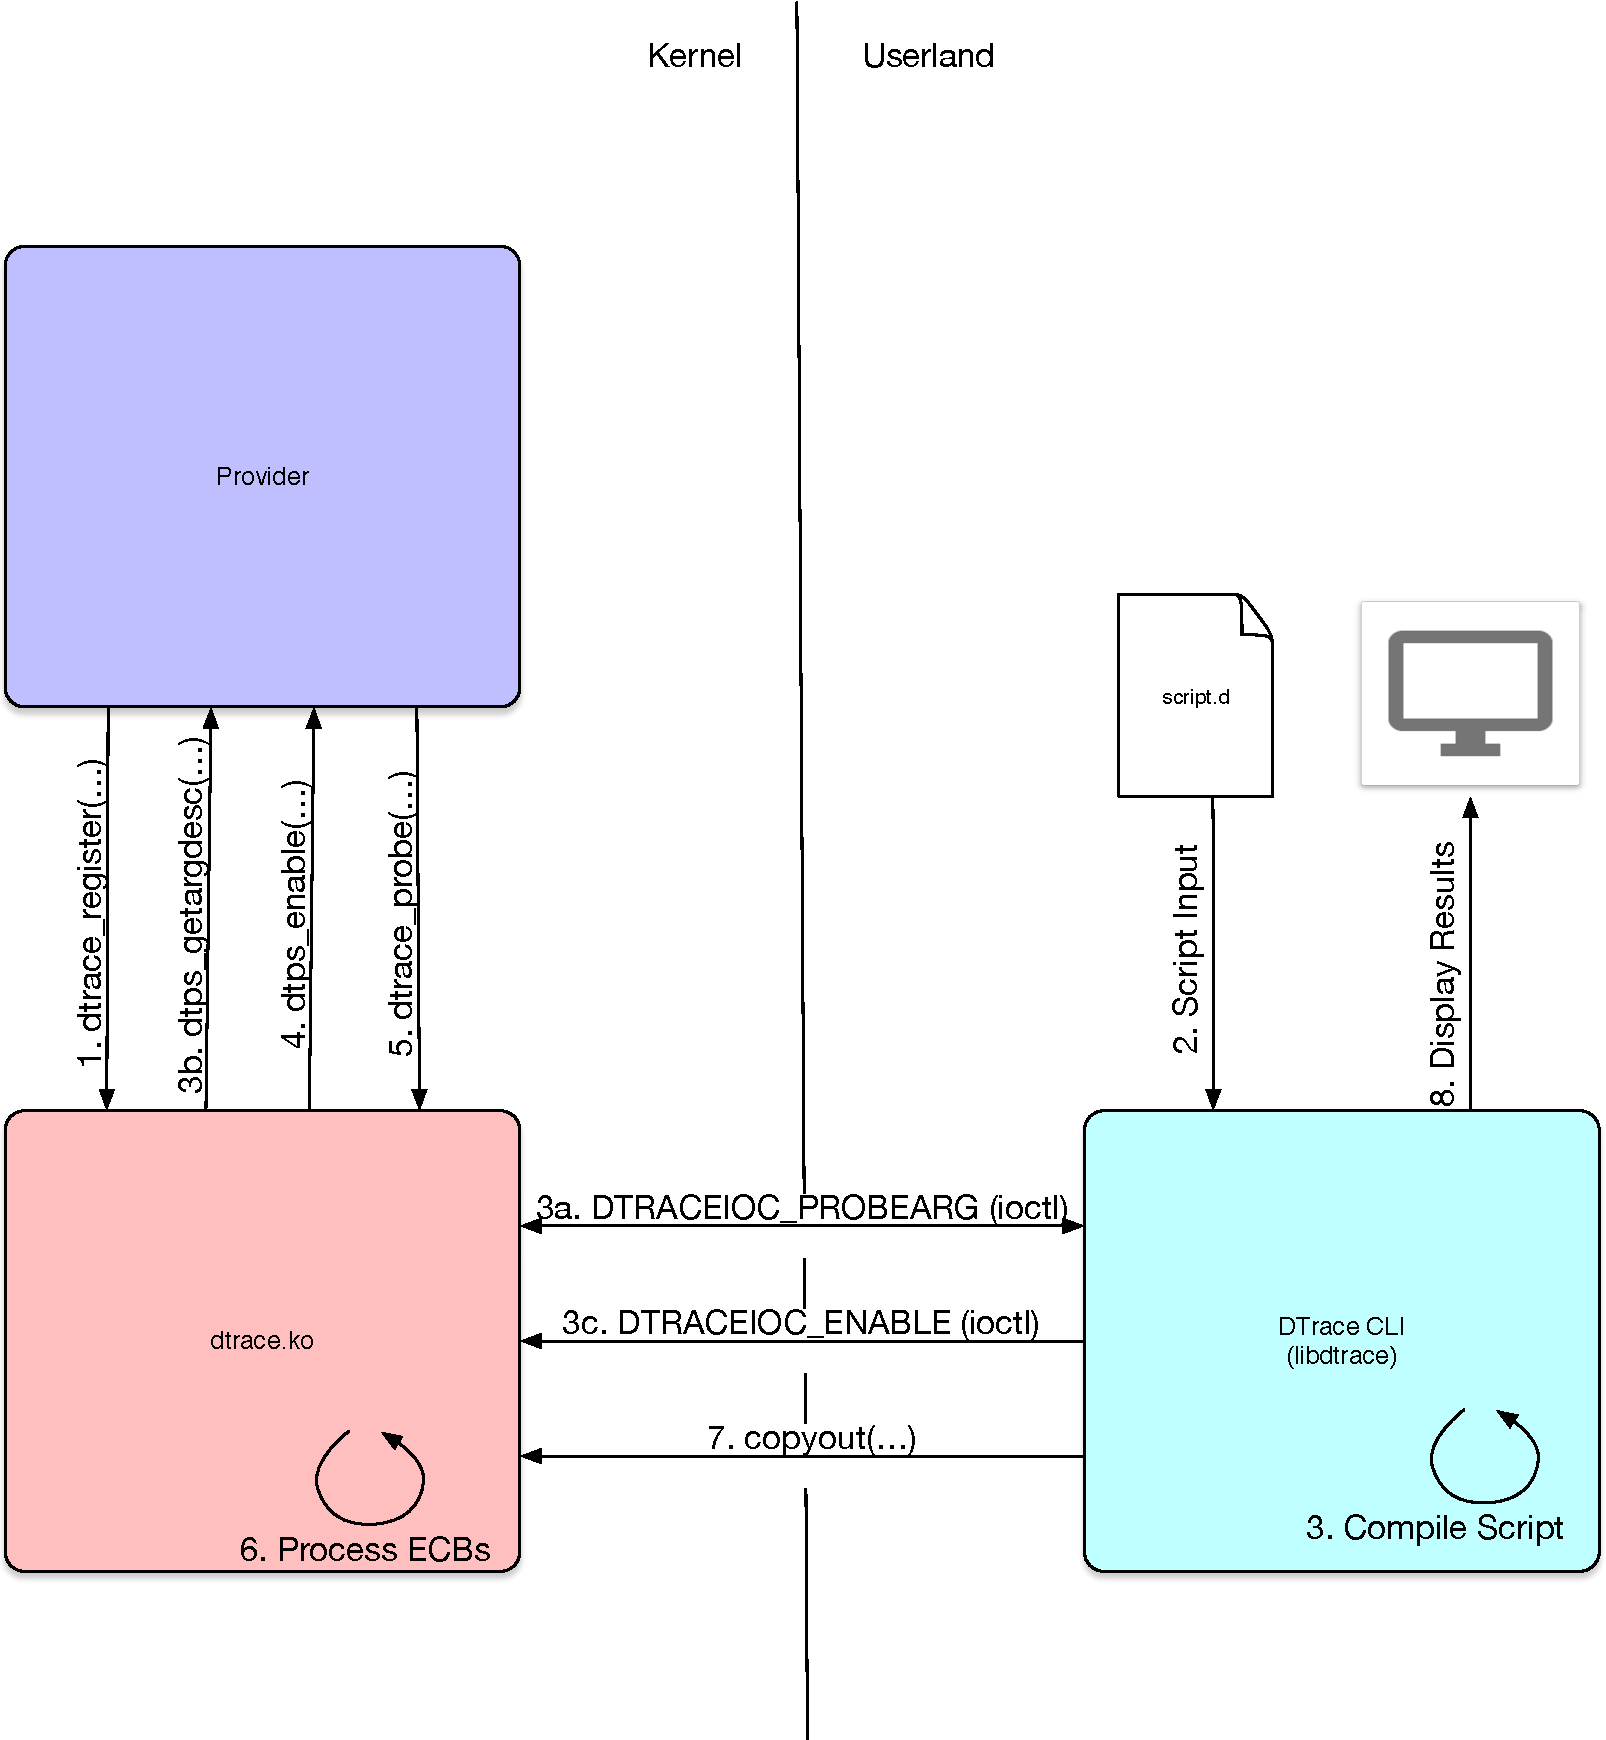
\includegraphics[width=0.8\linewidth]{dtrace-lifecycle.pdf}
	\caption{Typical lifecycle of an instrumentation using DTrace}
	\label{fig:lifecycle}
\end{figure}

When a provider is first loaded it registers itself with the
OpenDTrace kernel module (1). The registration process causes the
provider to enumerate all of its available probes, which are also
disabled by default.

The provider and kernel module remain idle until instrumentation is
requested. Instrumentation is requested via the \texttt{dtrace}
command in cooperation with the \texttt{libdtrace} library.  The the
user provides a D script, specifying the code to be run when a probe
fires (2). When the \texttt{dtrace} command executes it initializes
the \texttt{libdtrace} library, which in turn causes the kernel module
to initialize its tracing state and set up memory buffers to stored
the trace data.

The \texttt{libdtrace} library then compiles the D script (3). As part
of this process the compiler queries the kernel module to determine
the arguments for probes of interest via an ioctl (3a). The kernel in
turn queries the provider for a description of the probe arguments
which are returned to the compiler.  If the arguments discovered by
the kernel module do not match those supplied in the D script the
compiler will signal an error and abort compilation of the D script.
If the script did not supply any type information, the compilation
will complete and any mismatch will result in a runtime error.

The result of the D script compilation is an Enabling Code Block
(ECB). The ECB is provided to the kernel module (3c) which stores it
with others in a tree like structure. Once the ECB is safely stored in
the kernel, the kernel module tells the provider to enable the probes
that are to be instrumented.

When code execution reaches a point that has an enabled probe, the
probe fires and a call is made into the kernel module (5). The kernel
module then walks through the tree of ECBs, executing any that match
the probe that was fired (6). The captured data is written into the
buffer created when \texttt{libdtrace} was initialized. At a later
point the data is copied out of the kernel by the library (7), and
then the final results are made available to the end user (8).

\section{Privilege Model}
\label{sec:privilege}

The OpenDTrace privilege model is relatively simple, any program that
wishes to trace another program must be running with \emph{root}
privileges.  Some operating systems, such as Illumos, provide a more
nuanced privilege model.

\section{Tracepoint Format}
\label{sec:tracepoint-format}

\section{User Space Tracing}
\label{sec:user-space}

%%% Local Variables:
%%% mode: latex
%%% TeX-master: "dtrace-specification"
%%% End:


\chapter{OpenDTrace Compact C Type Format (CTF)}
\label{chap:opendtrace-ctf}
The Compact C Type Format (CTF) encapsulates all of the information
needed by OpenDTrace to understand C language types such as integers,
strings, floats and structures.  The goal of having another section
just for C type information is to provide a compact representation of
the information that usually appears in the debugging sections of
object files and executables.  CTF only contains data types it
does not contain other debugging infromation, which allows it to be
far more compact.  The debugging sections on a debug build of FreeBSD
in 2017 take up 78 megabytes of space, while the CTF section in the
same kernel take up only 800 kilobytes. 

\section{On Disk Format}
\label{sec:ctf-on-disk-format}

CTF data is stored in its own ELF section within an object file or
executable.  It is meant to be stored in a format that is both compact
and which is properly aligned so that it can be accessed using the
mmap(2) system call.

\begin{figure}[h]
  \centering
  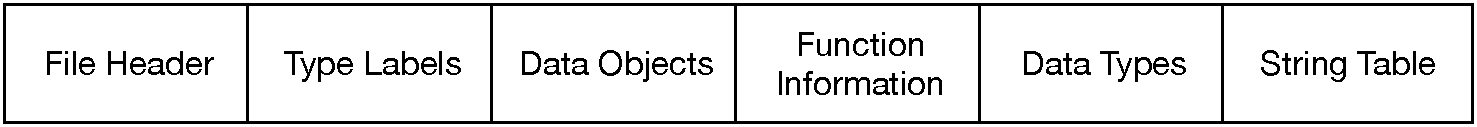
\includegraphics[width=.8\textwidth]{ctf-stable-format}
  \caption{CTF Stable Storage Format}
  \label{fig:ctf-stable-storage-format}
\end{figure}

Figure~\ref{fig:ctf-stable-storage-format} shows all of the components
of the CTF section as they would be found on stable storage.  The file
header stores a magic number and version information, encoding flags,
and the byte offset of each of the sections relative to the end of the
header itself.  As of this writing the most current version of CTF is
version two (2).  The preamble, including the magic number, version
and flags, take up the first 32 bits of the header, the remaining
fields take up 32 bits each, independent of the word size of the
architecture.

\begin{figure}
  \centering
  \begin{bytefield}[endianness=big,bitformatting=\scriptsize]{32}
    \bitheader{0,8,16,31} \\
    \bitbox{16}{magic}
    \bitbox{8}{version}
    \bitbox{8}{flags}\\
    \bitbox{32}{reference to parent label}\\
    \bitbox{32}{reference to basename of parent}\\
    \bitbox{32}{label section offset}\\
    \bitbox{32}{function section offset}\\
    \bitbox{32}{type section offset}\\
    \bitbox{32}{string section offset}\\
    \bitbox{32}{size of string section (bytes)}\\
  \end{bytefield}
  \caption{Overall CTF section encoding}
  \label{fig:ctf-overall}
\end{figure}

The CTF section makes heavy use of references between the sub-sections
to fully describe the datatypes in a program as well as the functions,
the function's argument list, and the function's return value.  The
\verb|data objects| and \verb|functions| sections depend upon the
\verb|type| section, which encodes all of the datatypes that have
been during the CTF conversion process.  Each type has a unique number
and name, as well as a size and encoding.  Types may refer to other,
more primitive types by use of a reference, e.g. a \verb|uint32_t|
will actually refer to a \verb|unsigned int|.  Types are broken up by
what they represent, referred to as their \emph{kind}.

\begin{table}
  \centering
  \begin{tabular}{|l|l|}
    \hline
    \verb|CTF_K_UNKNOWN|    & unknown type (used for padding) \\
    \verb|CTF_K_INTEGER|    & variant data is \verb|CTF_INT_DATA()| (see below)\\
    \verb|CTF_K_FLOAT|      & variant data is \verb|CTF_FP_DATA()| (see below)\\
    \verb|CTF_K_POINTER|    & \verb|ctt_type| is referenced type\\
    \verb|CTF_K_ARRAY|      & variant data is single \verb|ctf_array_t|\\
    \verb|CTF_K_FUNCTION| & \verb|ctt_type| is return type\\
                            &  variant data is list of argument types\\
                            & (\verb|ushort_t|'s)\\
    \verb|CTF_K_STRUCT|     & variant data is list of \verb|ctf_member_t|'s\\
    \verb|CTF_K_UNION|      & variant data is list of \verb|ctf_member_t|'s\\
    \verb|CTF_K_ENUM|       & variant data is list of \verb|ctf_enum_t|'s\\
    \verb|CTF_K_FORWARD|    & no additional data; \verb|ctt_name| is tag\\
    \verb|CTF_K_TYPEDEF|    & \verb|ctt_type| is referenced type\\
    \verb|CTF_K_VOLATILE|   & \verb|ctt_type| is base type\\
    \verb|CTF_K_CONST|      & \verb|ctt_type| is base type\\
    \verb|CTF_K_RESTRICT|   & \verb|ctt_type| is base type\\
    \hline
  \end{tabular}
  \caption{Kinds of CTF Base Types}
  \label{tbl:ctf-kinds}
\end{table}

Table\ref{tbl:ctf-kinds} lists the kinds of base data types that are
encoded by CTF.  Complex data types, such as structures, are also
contained in the \verb|types| section, and are encoded as a structure
with a name that references the string table.

\begin{figure}
  \centering
  \begin{bytefield}[endianness=big,bitformatting=\scriptsize]{32}
    \bitheader{0,16,31} \\
    \bitbox{32}{name}\\
    \bitbox{16}{info}
    \bitbox{16}{size or type}\\
  \end{bytefield}
  \caption{A simple type}
  \label{fig:ctf-stype}
\end{figure}

A simple type, one who's size is less than 64 Kbytes, is stored in a
\verb|ctf_stype|, Figure~\ref{fig:ctf-stype}.  The \verb|name| is a
reference to a string in the string table.  The \verb|info| field is
encoded differently for each type, as will be explained fully in the
rest of this chapter.  The last field is either the size, in bytes, of
the structure or it is a reference to another type, encoded using the
referenced type's ID.  The majority of types in a C program will fit
within a \verb|ctf_stype|.

\begin{figure}
  \centering
  \begin{bytefield}[endianness=big,bitformatting=\scriptsize]{32}
    \bitheader{0,16,31} \\
    \bitbox{32}{name}\\
    \bitbox{16}{info}
    \bitbox{16}{size or type}\\
    \bitbox{32}{high 32 bits of size (in bytes)}\\
    \bitbox{32}{low 32 bits of size (in bytes)}\\
  \end{bytefield}
  \caption{A large type}
  \label{fig:ctf-type}
\end{figure}

Types that are larger than 64Kbytes are encoded using a
\verb|ctf_type| structure, shown in Figure~\ref{fig:ctf-type}.  The
\verb|name| and \verb|info| fields of this, larger, \verb|ctf_type|
are the same as the smaller \verb|ctf_stype|, but the \verb|size|
field is always set to \verb|CTF_LSIZE_SENT|, the sentinal value that
tells the consumer that this is a larger structure.  A \verb|ctf_type|
structure can encode an extremely large type, since it provides 64
bits for the size, and that size is expressed in bytes.

\begin{figure}
  \centering
  \begin{bytefield}[endianness=big,bitformatting=\scriptsize]{16}
    \bitheader{0,9,10,15}\\
    \bitbox{5}{kind}
    \bitbox{1}{r}
    \bitbox{10}{vlen}
  \end{bytefield}
  \caption{Info field encoding}
  \label{fig:ctf-info-field}  
\end{figure}

The \verb|info| field, shown in Figure\ref{fig:ctf-info-field}, is
further broken down into a number of sub-fields which encoded the
\verb|kind|, \verb|vlen| (variable length) and whether or not this is
a root type \verb|isroot|.

Each of the integral types, such as integers, floats, pointers, arrays, etc.
has its own encoding.  Integers are the simplest type and are unsigned by
default.  An integer type is encoded in a single, 32 bit, field, as
seen in Figure~\ref{fig:ctf-integral}.

\begin{figure}
  \centering
  \begin{bytefield}[endianness=big,bitformatting=\scriptsize]{32}
    \bitheader{0,16,24,31} \\
    \bitbox{8}{flags}
    \bitbox{8}{offset}
    \bitbox{16}{size in bits}
  \end{bytefield}
  \caption{Integral type encoding}
  \label{fig:ctf-integral}
\end{figure}

The \verb|flags| field indicates whether the integer is signed,
contains character data, is a boolean or is to be displayed
with a varags style of formatting.

Floating point numbers have the exact same fields to describe them
but a larger number of possible flags, to match the larger
number of ways in which floating point numbers may be stored.
The flags and descriptions of the currently supported floating
point encodings are given in Table~\ref{tbl:ctf-kinds}.

\begin{table}
  \centering
  \begin{tabular}{|l|l|}
    \hline
    \verb|CTF_FP_SINGLE|   & IEEE 32-bit float encoding\\
    \verb|CTF_FP_DOUBLE|   & IEEE 64-bit float encoding\\
    \verb|CTF_FP_CPLX|     & Complex encoding\\
    \verb|CTF_FP_DCPLX|    & Double complex encoding\\
    \verb|CTF_FP_LDCPLX|   & Long double complex encoding\\
    \verb|CTF_FP_LDOUBLE|  & Long double encoding\\
    \verb|CTF_FP_INTRVL|   & Interval (2x32-bit) encoding\\
    \verb|CTF_FP_DINTRVL|  & Double interval (2x64-bit) encoding\\
    \verb|CTF_FP_LDINTRVL| & Long double interval (2x128-bit) encoding\\
    \verb|CTF_FP_IMAGRY|   & Imaginary (32-bit) encoding\\
    \verb|CTF_FP_DIMAGRY|  & Long imaginary (64-bit) encoding\\
    \verb|CTF_FP_LDIMAGRY| & Long long imaginary (128-bit) encoding\\
    \hline
  \end{tabular}
  \caption{Floating Point Encodings for CTF}
  \label{tbl:ctf-fp}
\end{table}

The functions section encodes the function name, as well as its arguments
and return value.  The types of the arguments and the return value
reference the \verb|types| section.  The arguments to the function
are encoded as a list.

All strings are encoded in the \verb|string table| and are referenced by
a numeric id from the other sections.

%%% Local Variables:
%%% mode: latex
%%% TeX-master: "dtrace-specification"
%%% End:


\chapter{OpenDTrace Object Format (DOF)}
\label{chap:opendtrace-object-format}
\section{Introduction}
\label{sec:dof-intro}

OpenDTrace programs are persistently encoded in the DOF format so that
they may be embedded in other programs (for example, in an ELF file)
or in the DTrace driver configuration file for use in anonymous
tracing.  The DOF format is versioned and extensible so that it can be
revised and so that internal data structures can be modified or
extended compatibly.  All DOF structures use fixed-size types, so the
32-bit and 64-bit representations are identical and consumers can use
either data model transparently.

\subsection{Stable Storage Format}
\label{sec:dof-stable-storage}

\begin{figure}[h]
  \centering
  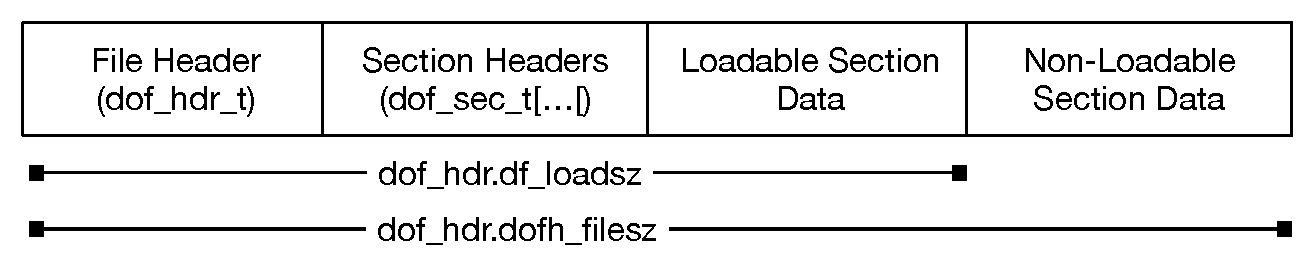
\includegraphics[width=.8\textwidth]{dof-stable-format}
  \caption{Stable Storage Format}
  \label{fig:dof-stable-storage-format}
\end{figure}

When a DOF file resides on stable storage it is stored in the format
shown in Figure~\ref{fig:dof-stable-storage-format}. The file header
stores meta-data including a magic number, data model for the
instrumentation, data encoding, and properties of the DIF code within.
The header describes its own size and the size of the section headers.
By convention, an array of section headers follows the file header,
and then the data for all loadable sections and sections which cannot
be loaded, also called unloadable sections.  This data layout permits
consumer code to easily download the headers and all loadable data
into the DTrace driver in one contiguous chunk, omitting other
extraneous sections.  DOF sections are used both for stable storage
and to pass data between user and kernel space, e.g. D programs are
sent into the kernel as a \verb|dof_prog_rt| section.

The section headers describe the size, offset, alignment, and section
type for each section.  Sections are described using a set of \verb|#defines|
that tell the consumer what kind of data is expected.  Sections can
contain links to other sections by storing a \verb|dof_secidx_t|, an index
into the section header array, inside of the section data structures.
The section header includes an entry size so that sections with data
arrays can grow their structures.

The DOF data itself can contain many snippets of DIF (i.e. more than
one DIF object or DIFO), which are represented themselves as a
collection of related DOF sections.  This allows us to change the set
of sections associated with a DIFO over time, and also allows us to
encode DIFOs that contain different sets of sections.  When a DOF
section wants to refer to a DIFO, it stores the \verb|dof_secidx_t| of
a section of type \verb|DOF_SECT_DIFOHDR|.  This section's data is
then an array of \verb|dof_secidx_t|'s which in turn denote the
sections associated with this DIFO.

This loose coupling of the file structure (header and sections) to the
structure of the DTrace program itself (enabling control block
descriptions, action descriptions, and DIFOs) permits activities such
as relocation processing to occur in a single pass without having to
understand D program structure.

Finally, strings are always stored in ELF-style string tables along
with a string table section index and string table offset.  Therefore
strings in DOF are always arbitrary-length and not bound to the
current implementation.

% Note from Samuel Lepetit
% A graph of which sections depend on which would be more useful I
% think here compared to just a list of sections (the dof.py lldb
% macros I wrote that you can find in the userspace Darwin repo are a
% bit easier to read than the code). Which sections are currently
% unused as well would be useful.

\begin{table}
  \centering
\begin{tabular}{|l|l|l|}
\hline
  Name & Loadable & Comment\\
\hline
\verb|DOF_SECT_NONE| & N & null section\\
\verb|DOF_SECT_COMMENTS| & N & compiler comments\\
\verb|DOF_SECT_SOURCE| & N & D program source code\\
\verb|DOF_SECT_ECBDESC| & Y & \verb|dof_ecbdesc_t|\\
\verb|DOF_SECT_PROBEDESC| & Y & \verb|dof_probedesc_t|\\
\verb|DOF_SECT_ACTDESC| & Y & \verb|dof_actdesc_t| array\\
\verb|DOF_SECT_DIFOHDR| & Y & \verb|dof_difohdr_t| (variable length)\\
\verb|DOF_SECT_DIF| & Y & \verb|uint32_t array| of byte code\\
\verb|DOF_SECT_STRTAB| & Y & string table\\
\verb|DOF_SECT_VARTAB| & Y & \verb|dtrace_difv_t| array\\
\verb|DOF_SECT_RELTAB| & Y & \verb|dof_relodesc_t| array\\
\verb|DOF_SECT_TYPTAB| & Y & \verb|dtrace_diftype_t| array\\
\verb|DOF_SECT_URELHDR| & Y & \verb|dof_relohdr_t| (user relocations)\\
\verb|DOF_SECT_KRELHDR| & Y & \verb|dof_relohdr_t| (kernel relocations)\\
\verb|DOF_SECT_OPTDESC| & Y & \verb|dof_optdesc_t| array\\
\verb|DOF_SECT_PROVIDER| & Y & \verb|dof_provider_t|\\
\verb|DOF_SECT_PROBES| & Y & \verb|dof_probe_t| array\\
\verb|DOF_SECT_PRARGS| & Y & \verb|uint8_t array| (probe arg mappings)\\
\verb|DOF_SECT_PROFFS| & Y & \verb|uint32_t array| (probe arg offsets)\\
\verb|DOF_SECT_INTTAB| & Y & \verb|uint64_t array|\\
\verb|DOF_SECT_UTSNAME| & N & \verb|struct utsname| structure\\
\verb|DOF_SECT_XLTAB| & Y & \verb|dof_xlref_t| array\\
\verb|DOF_SECT_XLMEMBERS| & Y & \verb|dof_xlmember_t| array\\
\verb|DOF_SECT_XLIMPORT| & Y & \verb|dof_xlator_t|\\
\verb|DOF_SECT_XLEXPORT| & Y & \verb|dof_xlator_t|\\
\verb|DOF_SECT_PREXPORT| & Y & \verb|dof_secidx_t| array (exported objs)\\
\verb|DOF_SECT_PRENOFFS| & Y & \verb|uint32_t array| (enabled offsets)\\
\hline
\end{tabular}
  \caption{DOF Section Descriptions}
  \label{tab:dof-sections}
\end{table}


%%% Local Variables:
%%% mode: latex
%%% TeX-master: "dtrace-specification"
%%% End:


\chapter{OpenDTrace Intermediate Format (DIF)}
\label{chap:opendtrace-intermediate-format}

\section{DTrace Instruction Version}

This specification describes the DTrace Intermediate Format version 2, as
shipped in Solaris \textbf{XXXRW}, FreeBSD \textbf{XXXRW}, and Mac OS X
\textbf{XXXRW}.

\section{The DIF Interpreter}

The DTrace Intermediate Format (DIF) interpreter executes instructions on behalf
of D scripts that are associated with predicates and actions.  DIF is a simple,
RISC-like, instruction set where each instruction consists of a 32-bit,
native-endian integer whose most significant 8 bits contain an opcode allowing
the remainder of the instruction to be decoded.  Interpretation is executed in a
loop within the \function{dtrace_dif_emulate} function, which has, as its first
argument, a pointer to a DIF Object or \struct{dtrace_difo_t}. Each of the DIF
Object gets executed in its own separtate environment and must return a value
using the \instruction{ret} instruction. Instructions are executed one at a
time, until they are exhausted or an error causes interpretation to end. The DIF
objects are verified in the \function{dtrace_difo_validate} function and the DIF
interpreter ignores any bounds checking within the \function{dtrace_dif_emulate}
function precisely because \function{dtrace_difo_validate} performs the
necessary checks.

\subsection{Registers}
\label{sec:dif-registers}

The DTrace virtual machine is made up of eight (8) integer registers
and eight (8) tuple registers.  The 0th integer register is always contains
the value zero (0).  All operations are carried out using registers
\registerop{r1} and \registerop{r2} as operands and \registerop{rd} as
the destination for all results.

\subsection{Math Instructions}
\label{sec:dif-math}

Instructions for mathematical operations in DIF have no concept of
over or underflow.  The division instructions set a flag to indicate a
division by zero error.

\subsection{Comparison and Test Instructions}
\label{sec:dif-cmp-tst}

\begin{table}
  \centering
    \begin{tabular}{|l|l|}
      \hline
      Variable & Meaning\\
      \hline
      cc\_r & Value of $r1 - r2$\\
      cc\_n & Comparison result is negative. \\
      cc\_z & Comparison result is 0.\\
      cc\_v & Overflow occurred.\\
      cc\_c & Is $r1 < r2$?\\
      \hline
  \end{tabular}
\label{tbl:cmp-vars}
\caption{Mathematical Operation Result Bits}
\end{table}

DIF has three instructions, \instruction{cmp}, \instruction{scmp} and
\instruction{tst} which can set various result flags, shown in
Table~\ref{tbl:cmp-vars}, which are later used by the branch
instructions.  The result flags are never returned directly to the
calling DIF program but are only used internally by the interpretation
routine.

\textbf{XXXRW: Something about instructions}

\subsection{Branching Instructions}

DIF has eleven split into two types: signed and unsigned branching instructions.
The signed branching instructions take into account that the number may be
negative, while the unsigned instructions are meant to be used with exclusively
positive numbers. One thing all of the branching instructions have in common is
that they load the new \register{pc} register from the \registerop{label} field
in the Branch Format described in Subsection~\ref{subsec:b-format}.

\subsection{Subroutine Calls}
\label{sec:subroutines}

DTrace provides an extensive set of subroutines for use by D programs.  The
subroutines are implemented within the kernel code via a set of functions which
are centrally dispatched from the \function{dtrace_dif_subr} function.  Within
DIF subroutines are triggered via the \instruction{CALL} instruction. The
arguments to these subroutines are passed through the tupregs variable through
use of the \instruction{PUSHTR} and \instruction{PUSHTV} instructions. The
return values of the subroutines are provided through the \registerop{rd}
register. The subroutine identifier is placed in the \registerop{idx} field of
the W-Format descrbied in Subsection~\ref{subsec:w-format}. Any subroutine that
is provided to DTrace \emph{must} go via these mechanisms.

\begin{quote}
  Notice that we don't bother validating the proper number of
  arguments or their types in the tuple stack.  This isn't needed
  because all argument interpretation is safe because of our load
  safety -- the worst that can happen is that a bogus program can
  obtain bogus results.
\label{fig:argcheck}
\end{quote}

According to a comment in the code, see Figure~\ref{fig:argcheck}, argument
checks are not carried out when a subroutine is called. These checks are
performed in the \function{dtrace_difo_validate} function at load time.

\textbf{XXXDS: Are these comments related to the Subroutine Calls section, or
overall?}

\textbf{XXXRW: Something about DIF registers, \nregs{}}

\textbf{XXXRW: Something about the zero register}

\textbf{XXXRW: Something about implied status bits}

\textbf{XXXRW: Something about scratch memory (alloca, user copyin)}

\textbf{XXXRW: Something about the tuple stack}

\textbf{XXXRW: Something about kernel memory access}

\textbf{XXXRW: Something about user memory access}

\textbf{XXXRW: Something about ``by reference''}

\textbf{XXXRW: Something about the integer table}

\textbf{XXXRW: Something about the string table}

\subsection{Local Variables}
\label{sec:local-vars}

Local variables are local to the D program clause.  In a D program
these variables are referenced using the \verb|this->| syntax.  

\subsection{Thread Local Variables}
\label{sec:thread-local-vars}

Thread local variables are usable in multiple D program clauses.  In a
D program the thread local variables are referenced using the
\verb|self->| syntax.

\subsection{Global Variables}
\label{sec:globals-vars}

Global variables are global to all the clauses in a D script and are references
to simple names within the D script.  Space for global variables is statically
allocated on each invocation of a script. Additionally, global variables are
identified using the modified register format as described in
Subsection~\ref{subsec:r-format} the case of arrays and the wide-immediate
format which is described in Subsection~\ref{subsec:w-format} in the case
of scalar variables inside of the \function{dtrace_dif_variable} function.

\textbf{XXXRW: Something about scalars}

\textbf{XXXRW: Something about arrays}

\textbf{XXXRW: Something about aggregations}

\textbf{XXXRW: Something about exceptions}

\section{Instruction Format}

Each instruction consists of a 32-bit, native-endian integer whose most
significant 8 bits contain an opcode allowing the remainder of the instruction
to be decoded.
To ease parsing, three major formats (R, B, and W) are used for all DTrace
instructions, capturing different types of operations: register-to-register
instructions accepting zero or more register operands; branch instructions
accepting a target label as a single operand; and wide-immediate instructions
that accept a 16-bit immediate used to capture both small constant values and
also indices into various tables.

\subsection{Register Format (R-Format)}
\label{subsec:r-format}
This format accepts zero or more register operands, supporting instructions
that include arithmetic and boolean operations, comparison and test
operations, load and store operations, tuple-stack operations, and the no-op
instruction.

\begin{center}
\begin{bytefield}[endianness=big,bitformatting=\scriptsize]{32}
\bitheader{0,7,8,15,16,23,24,31}\\
\bitbox{8}{op}
\bitbox{8}{r1}
\bitbox{8}{r2}
\bitbox{8}{rd}
\end{bytefield}
\end{center}

\begin{description}
\item[op] Mandatory 8-bit operation identifier
\item[r1, r2] Optional source registers providing input values to the
  operation
\item[rd] Optional destination register acting as the destination of the
  operation
\end{description}


A modified version of the Register Format is used when loading and
storing data in array variables in DTrace. The main difference between the
regular Register Format and the modified one used for arrays, is that the
\registerop{r1} register location is used as the variable identificator, the
\registerop{r2} register itself contains the optional index in the array.

\begin{center}
\begin{bytefield}[endianness=big,bitformatting=\scriptsize]{32}
\bitheader{0,7,8,15,16,23,24,31}\\
\bitbox{8}{op}
\bitbox{8}{var}
\bitbox{8}{r2}
\bitbox{8}{rd}
\end{bytefield}
\end{center}

\begin{description}
\item[op] Mandatory 8-bit operation identifier
\item[var] The variable identifier
\item[r2] Optional register that contains the index of the array
\item[rd] Optional destination register acting as the destination of the
  operation
\end{description}

\subsection{Branch Format (B-Format)}
\label{subsec:b-format}

This format accepts a single 24-bit integer operand identifying the label that
is the branch target.
It is used solely for the \textbf{BRANCH} instruction.

\begin{center}
\begin{bytefield}[endianness=big,bitformatting=\scriptsize]{32}
\bitheader{0,23,24,31}\\
\bitbox{8}{op}
\bitbox{24}{label}
\end{bytefield}
\end{center}

\begin{description}
\item[op] Mandatory 8-bit operation identifier
\item[label] Mandatory 24-bit integer label
\end{description}

\subsection{Wide-Immediate Format (W-Format)}
\label{subsec:w-format}

This format accepts an 8-bit register and 16-bit integer argument (frequently an
index).  It is used for a range of instructions including those to load values
from integer and string constant tables, as well as those that store scalar
values in variables. In addition to that, it is used in the \instruction{CALL}
instruction in order to specify the \registerop{rd} register and the subroutine
identifier.

\begin{center}
\begin{bytefield}[endianness=big,bitformatting=\scriptsize]{32}
\bitheader{0,7,8,23,24,31}\\
\bitbox{8}{op}
\bitbox{16}{idx}
\bitbox{8}{rs\textbar rd}
\end{bytefield}
\end{center}

\begin{description}
\item[op] Mandatory 8-bit operation identifier
\item[idx] Mandatory 16-bit integer index
\item[rs\textbar rd] Optional 8-bit register acting as the source or
  destination of the operation
\end{description}

\section{Instructions}

Chapter~\ref{chap:opendtrace-instruction-reference} contains a comprehensive
description of DTrace's instructions.

\section{Subroutines}

Chapter~\ref{chap:opendtrace-subroutines} contains a comprehensive description of
DTrace's built-in subroutines.


\chapter{OpenOpendtrace Instruction Reference}
\label{chap:opendtrace-instruction-reference}
This chapter describes the DTrace instruction set.  For a discussion
of the DIF interpreter as well as an overview of how these
instructions are handled see
Chapter~\ref{chap:opendtrace-intermediate-format}.

\section{Instruction List}
\label{sec:instruction-list}

\begin{table}
\begin{center}
\begin{tabular}{llp{11cm}}
\toprule
  Name & Opcode & Description \\
\midrule
  \hyperref[insn:or]{\instruction{OR}} & 1 & Bitwise Or \\
  \hyperref[insn:xor]{\instruction{XOR}} & 2 & Bitwise Exclusive Or \\
  \hyperref[insn:and]{\instruction{AND}} & 3 & Bitwise And \\
  \hyperref[insn:sll]{\instruction{SLL}} & 4 & Shift Left Logical \\
  \hyperref[insn:srl]{\instruction{SRL}} & 5 & Shift Right Logical \\
  \hyperref[insn:sub]{\instruction{SUB}} & 6 & Subtract \\
  \hyperref[insn:add]{\instruction{ADD}} & 7 & Add \\
  \hyperref[insn:mul]{\instruction{MUL}} & 8 & Multiply \\
  \hyperref[insn:sdiv]{\instruction{SDIV}} & 9 & Divide (Signed) \\
  \hyperref[insn:udiv]{\instruction{UDIV}} & 10 & Divide (Unsigned) \\
  \hyperref[insn:srem]{\instruction{SREM}} & 11 & Remainder (Unsigned) \\
  \hyperref[insn:urem]{\instruction{UREM}} & 12 & Remainder (Signed) \\
  \hyperref[insn:not]{\instruction{NOT}} & 13 & Bitwise Not \\
  \hyperref[insn:mov]{\instruction{MOV}} & 14 & Move \\
  \hyperref[insn:cmp]{\instruction{CMP}} & 15 & Compare \\
  \hyperref[insn:tst]{\instruction{TST}} & 16 & Test Equal to Zero \\
\midrule
  & & See Table~\ref{tbl:b-format-instr} \\
\midrule
  \hyperref[insn:ldsb]{\instruction{LDSB}} & 28 & Load Byte (Signed) \\
  \hyperref[insn:ldsh]{\instruction{LDSH}} & 29 & Load Halfword (Signed) \\
  \hyperref[insn:ldsw]{\instruction{LDSW}} & 30 & Load Word (Signed) \\
  \hyperref[insn:ldub]{\instruction{LDUB}} & 31 & Load Byte (Unsigned) \\
  \hyperref[insn:lduh]{\instruction{LDUH}} & 32 & Load Halfword (Unsigned) \\
  \hyperref[insn:lduw]{\instruction{LDUW}} & 33 & Load Word (Unsigned) \\
  \hyperref[insn:ldx]{\instruction{LDX}} & 34 & Load Doubleword \\
  \hyperref[insn:ret]{\instruction{RET}} & 35 & Return \\
  \hyperref[insn:nop]{\instruction{NOP}} & 36 & No Operation \\
\midrule
  & & See Table~\ref{tbl:w-format-instr} \\
\midrule
  \hyperref[insn:scmp]{\instruction{SCMP}} & 39 & String Compare \\
  \hyperref[insn:ldga]{\instruction{LDGA}} & 40 & Load from Global Array \\
  \hyperref[insn:ldgs]{\instruction{LDGS}} & 41 & Load from Global Scalar \\
  \hyperref[insn:stgs]{\instruction{STGS}} & 42 & Store to Global Scalar \\
  \hyperref[insn:ldta]{\instruction{LDTA}} & 43 & Load from Thread-Local Array \\
  \hyperref[insn:ldts]{\instruction{LDTS}} & 44 & Load from Thread-Local Scalar \\
  \hyperref[insn:stts]{\instruction{STTS}} & 45 & Store to Thread-Local Scalar \\
  \hyperref[insn:sra]{\instruction{SRA}} & 46 & Shift Right Arithmatic \\
\bottomrule
\end{tabular}
\end{center}
\caption{R-Format Instruction List (Part 1)}
\label{tbl:r-format-instr-1}
\end{table}

\begin{table}
\begin{center}
\begin{tabular}{llp{11cm}}
\toprule
  Name & Opcode & Description \\
\midrule
  \hyperref[insn:pushtr]{\instruction{PUSHTR}} & 48 & Push a reference onto the tuple stack \\
  \hyperref[insn:pushtv]{\instruction{PUSHTV}} & 49 & Push a value onto the tuple stack \\
  \hyperref[insn:popts]{\instruction{POPTS}} & 50 & Pop the tuple stack \\
  \hyperref[insn:flushts]{\instruction{FLUSHTS}} & 51 & Flush the tuple stack \\
\midrule
  & & See Table \ref{tbl:w-format-instr}\\
\midrule
  \hyperref[insn:allocs]{\instruction{ALLOCS}} & 58 & Allocate scratch space \\
  \hyperref[insn:copys]{\instruction{COPYS}} & 59 & Copy memory of requested size \\
  \hyperref[insn:stb]{\instruction{STB}} & 60 & Store byte \\
  \hyperref[insn:sth]{\instruction{STH}} & 61 & Store halfword \\
  \hyperref[insn:stw]{\instruction{STW}} & 62 & Store word \\
  \hyperref[insn:stx]{\instruction{STX}} & 63 & Store doubleword \\
  \hyperref[insn:uldsb]{\instruction{ULDSB}} & 64 & Load user byte (signed) \\
  \hyperref[insn:uldsh]{\instruction{ULDSH}} & 65 & Load user halfword (signed) \\
  \hyperref[insn:uldsw]{\instruction{ULDSW}} & 66 & Load user word (signed) \\
  \hyperref[insn:uldub]{\instruction{ULDUB}} & 67 & Load user byte (unsigned) \\
  \hyperref[insn:ulduh]{\instruction{ULDUH}} & 68 & Load user halfword (signed) \\
  \hyperref[insn:ulduw]{\instruction{ULDUW}} & 69 & Load user word (signed) \\
  \hyperref[insn:uldx]{\instruction{ULDX}} & 70 & Load user doubleword \\
  \hyperref[insn:rldsb]{\instruction{RLDSB}} & 71 & If accessible, load byte (signed) \\
  \hyperref[insn:rldsh]{\instruction{RLDSH}} & 72 & If accessible, load halfword (signed) \\
  \hyperref[insn:rldsw]{\instruction{RLDSW}} & 73 & If accessible, load word (signed) \\
  \hyperref[insn:rldub]{\instruction{RLDUB}} & 74 & If accessible, load byte (unsigned) \\
  \hyperref[insn:rlduh]{\instruction{RLDUH}} & 75 & If accessible, load halfword (unsigned) \\
  \hyperref[insn:rlduw]{\instruction{RLDUW}} & 75 & If accessible, load word (unsigned) \\
  \hyperref[insn:rldx]{\instruction{RLDX}} & 77 & If accessible, load doubleword \\
\bottomrule
\end{tabular}
\end{center}
\caption{R-Format Instruction List (Part 2)}
\label{tbl:r-format-instr-2}
\end{table}

\begin{table}
\begin{center}
\begin{tabular}{llp{11cm}}
\toprule
  Name & Opcode & Description \\
\midrule
  \hyperref[insn:ba]{\instruction{BA}} & 17 & Unconditional branch \\
  \hyperref[insn:be]{\instruction{BE}} & 18 & Branch if equal to zero \\
  \hyperref[insn:bne]{\instruction{BNE}} & 19 & Branch if not equal to zero \\
  \hyperref[insn:bg]{\instruction{BG}} & 20 & Branch if greater than (signed) \\
  \hyperref[insn:bgu]{\instruction{BGU}} & 21 & Branch if greater than (unsigned) \\
  \hyperref[insn:bge]{\instruction{BGE}} & 22 & Branch if greater than or equal to (signed) \\
  \hyperref[insn:bgeu]{\instruction{BGEU}} & 23 & Branch if greater than or equal to (unsigned) \\
  \hyperref[insn:bl]{\instruction{BL}} & 24 & Branch if less than (signed) \\
  \hyperref[insn:blu]{\instruction{BLU}} & 25 & Branch if less than (unsigned) \\
  \hyperref[insn:ble]{\instruction{BLE}} & 26 & Branch if less than or equal to (signed) \\
  \hyperref[insn:bleu]{\instruction{BLEU}} & 27 & Branch if less than or equal to (unsigned) \\
\bottomrule
\end{tabular}
\end{center}
\caption{B-Format Instruction List}
\label{tbl:b-format-instr}
\end{table}

\begin{table}
\begin{center}
\begin{tabular}{llp{11cm}}
\toprule
  Name & Opcode & Description \\
\midrule
  \hyperref[insn:setx]{\instruction{SETX}} & 37 & Set register from integer table \\
  \hyperref[insn:sets]{\instruction{SETS}} & 38 & Set register from string table \\
\midrule
  \hyperref[insn:call]{\instruction{CALL}} & 47 & Call subroutine \\
\midrule
  \hyperref[insn:ldgaa]{\instruction{LDGAA}} & 52 & Load from global aggregation \\
  \hyperref[insn:ldtaa]{\instruction{LDTAA}} & 53 & Load from thread-local aggregation \\
  \hyperref[insn:stgaa]{\instruction{STGAA}} & 54 & Store to global aggregation \\
  \hyperref[insn:sttaa]{\instruction{STTAA}} & 55 & Store to thread-local aggregation \\
  \hyperref[insn:ldls]{\instruction{LDLS}} & 56 & Load from local scalar \\
  \hyperref[insn:stls]{\instruction{STLS}} & 57 & Store to local scalar \\
\midrule
  \hyperref[insn:xlate]{\instruction{XLATE}} & 78 & \textbf{Illumos Only} \\
  \hyperref[insn:xlarg]{\instruction{XLARG}} & 79 & \textbf{Illumos Only} \\
\bottomrule
\end{tabular}
\end{center}
\caption{W-Format Instruction List}
\label{tbl:w-format-instr}
\end{table}

\newpage
\section{Individual Instructions}

\clearpage
\phantomsection
\addcontentsline{toc}{subsection}{AND}
\label{insn:and}
\subsection*{AND: Bitwise And}

\subsubsection*{Format}

\textrm{AND \%rd, \%r1, \%r2}

\begin{center}
\begin{bytefield}[endianness=big,bitformatting=\scriptsize]{32}
\bitheader{0,7,8,15,16,23,24,31} \\
\bitbox{8}{0x03}
\bitbox{8}{r1}
\bitbox{8}{r2}
\bitbox{8}{rd}
\end{bytefield}
\end{center}

\subsubsection*{Description}

This instruction calculates the bitwise and of the values found in registers
\registerop{r1} and \registerop{r2}, placing the results in register
\registerop{rd}.

\subsubsection*{Pseudocode}

\begin{verbatim}
regs[rd] = regs[r1] & regs[r2]
\end{verbatim}

\subsubsection*{Constraints}

\registerop{r1}, \registerop{r2}, and \registerop{rd} must be less than
\nregs{}.

\medskip
\noindent
\registerop{rd} cannot be \register{r0}.

\subsubsection*{Failure modes}

This instruction has no run-time failure modes beyond its constraints.

\clearpage
\phantomsection
\addcontentsline{toc}{subsection}{OR}
\label{insn:or}
\subsection*{OR: Bitwise Or}

\subsubsection*{Format}

\textrm{OR \%rd, \%r1, \%r2}

\begin{center}
\begin{bytefield}[endianness=big,bitformatting=\scriptsize]{32}
\bitheader{0,7,8,15,16,23,24,31} \\
\bitbox{8}{0x01}
\bitbox{8}{r1}
\bitbox{8}{r2}
\bitbox{8}{rd}
\end{bytefield}
\end{center}

\subsubsection*{Description}

This instruction calculates the bitwise or of the values found in registers
\register{r1} and \register{r2}, placing the results in register
\register{rd}.

\subsubsection*{Pseudocode}

\begin{verbatim}
%rd = %r1 | %r2
\end{verbatim}

\subsubsection*{Constraints}

\registerop{r1}, \registerop{r2}, and \registerop{rd} must be less than
\nregs{}.

\medskip
\noindent
\registerop{rd} cannot be \register{r0}.

\subsubsection*{Failure modes}

This instruction has no run-time failure modes beyond its constraints.

\clearpage
\phantomsection
\addcontentsline{toc}{subsection}{SLL}
\label{insn:sll}
\subsection*{SLL: Shift Left Logical}

\subsubsection*{Format}

\textrm{SLL \%rd, \%r1, \%r2}

\begin{center}
\begin{bytefield}[endianness=big,bitformatting=\scriptsize]{32}
\bitheader{0,7,8,15,16,23,24,31} \\
\bitbox{8}{0x04}
\bitbox{8}{r1}
\bitbox{8}{r2}
\bitbox{8}{rd}
\end{bytefield}
\end{center}

\subsubsection*{Description}

This instruction shifts the value found in regiseter \register{r1} left by the
number of bits found in register \register{r2}, placing the results in
register \register{rd}.

\subsubsection*{Pseudocode}

\begin{verbatim}
%rd = %r1 << %r2
\end{verbatim}

\subsubsection*{Constraints}

\registerop{r1}, \registerop{r2}, and \registerop{rd} must be less than
\nregs{}.

\medskip
\noindent
\registerop{rd} cannot be \register{r0}.

\subsubsection*{Failure modes}

This instruction has no run-time failure modes beyond its constraints.

\clearpage
\phantomsection
\addcontentsline{toc}{subsection}{SRL}
\label{insn:srl}
\subsection*{SRL: Shift Right Logical}

\subsubsection*{Format}

\textrm{SRL \%rd, \%r1, \%r2}

\begin{center}
\begin{bytefield}[endianness=big,bitformatting=\scriptsize]{32}
\bitheader{0,7,8,15,16,23,24,31} \\
\bitbox{8}{0x05}
\bitbox{8}{r1}
\bitbox{8}{r2}
\bitbox{8}{rd}
\end{bytefield}
\end{center}

\subsubsection*{Description}

This instruction shifts the value found in regiseter \register{r1} right by
the number of bits found in register \register{r2}, placing the results in
register \register{rd}.

\subsubsection*{Pseudocode}

\begin{verbatim}
%rd = %r1 >> %r2
\end{verbatim}

\subsubsection*{Constraints}

\registerop{r1}, \registerop{r2}, and \registerop{rd} must be less than
\nregs{}.

\medskip
\noindent
\registerop{rd} cannot be \register{r0}.

\subsubsection*{Failure modes}

This instruction has no run-time failure modes beyond its constraints.

\clearpage
\phantomsection
\addcontentsline{toc}{subsection}{XOR}
\label{insn:or}
\subsection*{XOR: Bitwise Or}

\subsubsection*{Format}

\textrm{XOR \%rd, \%r1, \%r2}

\begin{center}
\begin{bytefield}[endianness=big,bitformatting=\scriptsize]{32}
\bitheader{0,7,8,15,16,23,24,31} \\
\bitbox{8}{0x02}
\bitbox{8}{r1}
\bitbox{8}{r2}
\bitbox{8}{rd}
\end{bytefield}
\end{center}

\subsubsection*{Description}

This instruction calculates the bitwise exclusive or of the values
found in registers \register{r1} and \register{r2}, placing the
results in register \register{rd}.

\subsubsection*{Pseudocode}

\begin{verbatim}
regs[rd] = regs[r1] ^ regs[r2]
\end{verbatim}

\subsubsection*{Constraints}

\registerop{r1}, \registerop{r2}, and \registerop{rd} must be less than
\nregs{}.

\medskip
\noindent
\registerop{rd} cannot be \register{r0}.

\subsubsection*{Failure modes}

This instruction has no run-time failure modes beyond its constraints.

\clearpage
\phantomsection
\addcontentsline{toc}{subsection}{SUB}
\label{insn:sub}
\subsection*{SUB: subtract the value in r2 from that in r1}

\subsubsection*{Format}

\textrm{SUB \%rd, \%r1, \%r2}

\begin{center}
\begin{bytefield}[endianness=big,bitformatting=\scriptsize]{32}
\bitheader{0,7,8,15,16,23,24,31} \\
\bitbox{8}{0x06}
\bitbox{8}{r1}
\bitbox{8}{r2}
\bitbox{8}{rd}
\end{bytefield}
\end{center}

\subsubsection*{Description}

The \instruction{sub} instruction takes the value in \registerop{r2}
and subtracts it from that in \registerop{r1} placing the result in
\registerop{rd}. 

\subsubsection*{Pseudocode}

\begin{verbatim}
%rd = %r1 - %r2
\end{verbatim}

\subsubsection*{Constraints}

\subsubsection*{Failure modes}

This instruction has no run-time failure modes beyond its constraints.

\clearpage
\phantomsection
\addcontentsline{toc}{subsection}{ADD}
\label{insn:add}
\subsection*{ADD: add two values}

\subsubsection*{Format}

\textrm{add \%r1, \%r2, \%rd}

\begin{center}
\begin{bytefield}[endianness=big,bitformatting=\scriptsize]{32}
\bitheader{0,7,8,15,16,23,24,31} \\
\bitbox{8}{0x07}
\bitbox{8}{r1}
\bitbox{8}{r2}
\bitbox{8}{rd}
\end{bytefield}
\end{center}

\subsubsection*{Description}
The \instruction{add} instruction adds the the values in
\registerop{r1} and \registerop{r2} and pace the results in register
\registerop{rd}.

\subsubsection*{Pseudocode}

\begin{verbatim}
regs[rd] = regs[r1] + regs[r2]
\end{verbatim}

\subsubsection*{Constraints}

\subsubsection*{Failure modes}

This instruction has no run-time failure modes beyond its constraints.

\clearpage
\phantomsection
\addcontentsline{toc}{subsection}{DUMMY}
\label{insn:dummy}
\subsection*{DUMMY: DUMMY}

\subsubsection*{Format}

\textrm{DUMMY \%rd, \%r1, \%r2}

\begin{center}
\begin{bytefield}[endianness=big,bitformatting=\scriptsize]{32}
\bitheader{0,7,8,15,16,23,24,31} \\
\bitbox{8}{0x01}
\bitbox{8}{r1}
\bitbox{8}{r2}
\bitbox{8}{rd}
\end{bytefield}
\end{center}

\subsubsection*{Description}

This instruction 
\subsubsection*{Pseudocode}

\begin{verbatim}
%rd = %r1 | %r2
\end{verbatim}

\subsubsection*{Constraints}

\subsubsection*{Failure modes}

This instruction has no run-time failure modes beyond its constraints.

\clearpage
\phantomsection
\addcontentsline{toc}{subsection}{SDIV}
\label{insn:sdiv}
\subsection*{SDIV: signed division}

\subsubsection*{Format}

\textrm{SDIV \%rd, \%r1, \%r2}

\begin{center}
\begin{bytefield}[endianness=big,bitformatting=\scriptsize]{32}
\bitheader{0,7,8,15,16,23,24,31} \\
\bitbox{8}{0x09}
\bitbox{8}{r1}
\bitbox{8}{r2}
\bitbox{8}{rd}
\end{bytefield}
\end{center}

\subsubsection*{Description}

The \instruction{sdiv} instruction divides the value contained in
\registerop{r2} into that contained in \registerop{r1} placing the
results into \registerop{rd}.  The values in both \registerop{r1} and
\registerop{r2} are first promoted to signed, 64 bit values, before
the division operation is carried out.

\subsubsection*{Pseudocode}

\begin{verbatim}
%rd = (int64_t)%r1 / (inst64_t)%r2
\end{verbatim}

\subsubsection*{Constraints}

\subsubsection*{Failure modes}

This instruction has no run-time failure modes beyond its constraints.

\clearpage
\phantomsection
\addcontentsline{toc}{subsection}{DUMMY}
\label{insn:dummy}
\subsection*{DUMMY: DUMMY}

\subsubsection*{Format}

\textrm{DUMMY \%rd, \%r1, \%r2}

\begin{center}
\begin{bytefield}[endianness=big,bitformatting=\scriptsize]{32}
\bitheader{0,7,8,15,16,23,24,31} \\
\bitbox{8}{0x01}
\bitbox{8}{r1}
\bitbox{8}{r2}
\bitbox{8}{rd}
\end{bytefield}
\end{center}

\subsubsection*{Description}

This instruction 
\subsubsection*{Pseudocode}

\begin{verbatim}
%rd = %r1 | %r2
\end{verbatim}

\subsubsection*{Constraints}

\subsubsection*{Failure modes}

This instruction has no run-time failure modes beyond its constraints.

\clearpage
\phantomsection
\addcontentsline{toc}{subsection}{SREM}
\label{insn:srem}
\subsection*{SREM: divide two numbers and store the remainder}

\subsubsection*{Format}

\textrm{SREM \%rd, \%r1, \%r2}

\begin{center}
\begin{bytefield}[endianness=big,bitformatting=\scriptsize]{32}
\bitheader{0,7,8,15,16,23,24,31} \\
\bitbox{8}{0x0B}
\bitbox{8}{r1}
\bitbox{8}{r2}
\bitbox{8}{rd}
\end{bytefield}
\end{center}

\subsubsection*{Description}

The \instruction{srem} instruction divides the value contained in
\registerop{r2} into that contained in \registerop{r1} placing the
remainder into \registerop{rd}.  The values in both \registerop{r1} and
\registerop{r2} are first promoted to signed, 64 bit values, before
the division operation is carried out.

\subsubsection*{Pseudocode}

\begin{verbatim}
regs[rd] = (int64_t)regs[r1] % (inst64_t)regs[r2]
\end{verbatim}

\subsubsection*{Constraints}

\subsubsection*{Failure modes}

This instruction has no run-time failure modes beyond its constraints.

\clearpage
\phantomsection
\addcontentsline{toc}{subsection}{DUMMY}
\label{insn:dummy}
\subsection*{DUMMY: DUMMY}

\subsubsection*{Format}

\textrm{DUMMY \%rd, \%r1, \%r2}

\begin{center}
\begin{bytefield}[endianness=big,bitformatting=\scriptsize]{32}
\bitheader{0,7,8,15,16,23,24,31} \\
\bitbox{8}{0x01}
\bitbox{8}{r1}
\bitbox{8}{r2}
\bitbox{8}{rd}
\end{bytefield}
\end{center}

\subsubsection*{Description}

This instruction 
\subsubsection*{Pseudocode}

\begin{verbatim}
%rd = %r1 | %r2
\end{verbatim}

\subsubsection*{Constraints}

\subsubsection*{Failure modes}

This instruction has no run-time failure modes beyond its constraints.

\clearpage
\phantomsection
\addcontentsline{toc}{subsection}{NOT}
\label{insn:not}
\subsection*{NOT: negate a value}

\subsubsection*{Format}

\textrm{NOT \%rd, \%r1}

\begin{center}
\begin{bytefield}[endianness=big,bitformatting=\scriptsize]{32}
\bitheader{0,7,8,15,16,23,24,31} \\
\bitbox{8}{0x0C}
\bitbox{8}{r1}
\bitbox{8}{r2}
\bitbox{8}{rd}
\end{bytefield}
\end{center}

\subsubsection*{Description}

The \instruction{not} instruction negates the value found in
\registerop{r1} and places the result into \registerop{rd}.
\subsubsection*{Pseudocode}

\begin{verbatim}
regs[rd] = ~regs[r1]
\end{verbatim}

\subsubsection*{Constraints}

\subsubsection*{Failure modes}

This instruction has no run-time failure modes beyond its constraints.

\clearpage
\phantomsection
\addcontentsline{toc}{subsection}{DUMMY}
\label{insn:dummy}
\subsection*{DUMMY: DUMMY}

\subsubsection*{Format}

\textrm{DUMMY \%rd, \%r1, \%r2}

\begin{center}
\begin{bytefield}[endianness=big,bitformatting=\scriptsize]{32}
\bitheader{0,7,8,15,16,23,24,31} \\
\bitbox{8}{0x01}
\bitbox{8}{r1}
\bitbox{8}{r2}
\bitbox{8}{rd}
\end{bytefield}
\end{center}

\subsubsection*{Description}

This instruction 
\subsubsection*{Pseudocode}

\begin{verbatim}
%rd = %r1 | %r2
\end{verbatim}

\subsubsection*{Constraints}

\subsubsection*{Failure modes}

This instruction has no run-time failure modes beyond its constraints.

\clearpage
\phantomsection
\addcontentsline{toc}{subsection}{DUMMY}
\label{insn:dummy}
\subsection*{DUMMY: DUMMY}

\subsubsection*{Format}

\textrm{DUMMY \%rd, \%r1, \%r2}

\begin{center}
\begin{bytefield}[endianness=big,bitformatting=\scriptsize]{32}
\bitheader{0,7,8,15,16,23,24,31} \\
\bitbox{8}{0x01}
\bitbox{8}{r1}
\bitbox{8}{r2}
\bitbox{8}{rd}
\end{bytefield}
\end{center}

\subsubsection*{Description}

This instruction 
\subsubsection*{Pseudocode}

\begin{verbatim}
%rd = %r1 | %r2
\end{verbatim}

\subsubsection*{Constraints}

\subsubsection*{Failure modes}

This instruction has no run-time failure modes beyond its constraints.

\clearpage
\phantomsection
\addcontentsline{toc}{subsection}{DUMMY}
\label{insn:dummy}
\subsection*{DUMMY: DUMMY}

\subsubsection*{Format}

\textrm{DUMMY \%rd, \%r1, \%r2}

\begin{center}
\begin{bytefield}[endianness=big,bitformatting=\scriptsize]{32}
\bitheader{0,7,8,15,16,23,24,31} \\
\bitbox{8}{0x01}
\bitbox{8}{r1}
\bitbox{8}{r2}
\bitbox{8}{rd}
\end{bytefield}
\end{center}

\subsubsection*{Description}

This instruction 
\subsubsection*{Pseudocode}

\begin{verbatim}
%rd = %r1 | %r2
\end{verbatim}

\subsubsection*{Constraints}

\subsubsection*{Failure modes}

This instruction has no run-time failure modes beyond its constraints.

\clearpage
\phantomsection
\addcontentsline{toc}{subsection}{BA}
\label{insn:dummy}
\subsection*{BA: branch absolute}

\subsubsection*{Format}

\textrm{BA label}

\begin{center}
\begin{bytefield}[endianness=big,bitformatting=\scriptsize]{32}
\bitheader{0,23,24,31} \\
\bitbox{8}{0x10}
\bitbox{24}{label}
\end{bytefield}
\end{center}

\subsubsection*{Description}

This instruction 
\subsubsection*{Pseudocode}

\begin{verbatim}
%pc = label
\end{verbatim}

\subsubsection*{Constraints}

\subsubsection*{Failure modes}

This instruction has no run-time failure modes beyond its constraints.

\clearpage
\phantomsection
\addcontentsline{toc}{subsection}{DUMMY}
\label{insn:dummy}
\subsection*{DUMMY: DUMMY}

\subsubsection*{Format}

\textrm{DUMMY \%rd, \%r1, \%r2}

\begin{center}
\begin{bytefield}[endianness=big,bitformatting=\scriptsize]{32}
\bitheader{0,7,8,15,16,23,24,31} \\
\bitbox{8}{0x01}
\bitbox{8}{r1}
\bitbox{8}{r2}
\bitbox{8}{rd}
\end{bytefield}
\end{center}

\subsubsection*{Description}

This instruction 
\subsubsection*{Pseudocode}

\begin{verbatim}
%rd = %r1 | %r2
\end{verbatim}

\subsubsection*{Constraints}

\subsubsection*{Failure modes}

This instruction has no run-time failure modes beyond its constraints.

\clearpage
\phantomsection
\addcontentsline{toc}{subsection}{DUMMY}
\label{insn:dummy}
\subsection*{DUMMY: DUMMY}

\subsubsection*{Format}

\textrm{DUMMY \%rd, \%r1, \%r2}

\begin{center}
\begin{bytefield}[endianness=big,bitformatting=\scriptsize]{32}
\bitheader{0,7,8,15,16,23,24,31} \\
\bitbox{8}{0x01}
\bitbox{8}{r1}
\bitbox{8}{r2}
\bitbox{8}{rd}
\end{bytefield}
\end{center}

\subsubsection*{Description}

This instruction 
\subsubsection*{Pseudocode}

\begin{verbatim}
%rd = %r1 | %r2
\end{verbatim}

\subsubsection*{Constraints}

\subsubsection*{Failure modes}

This instruction has no run-time failure modes beyond its constraints.

\clearpage
\phantomsection
\addcontentsline{toc}{subsection}{DUMMY}
\label{insn:dummy}
\subsection*{DUMMY: DUMMY}

\subsubsection*{Format}

\textrm{DUMMY \%rd, \%r1, \%r2}

\begin{center}
\begin{bytefield}[endianness=big,bitformatting=\scriptsize]{32}
\bitheader{0,7,8,15,16,23,24,31} \\
\bitbox{8}{0x01}
\bitbox{8}{r1}
\bitbox{8}{r2}
\bitbox{8}{rd}
\end{bytefield}
\end{center}

\subsubsection*{Description}

This instruction 
\subsubsection*{Pseudocode}

\begin{verbatim}
%rd = %r1 | %r2
\end{verbatim}

\subsubsection*{Constraints}

\subsubsection*{Failure modes}

This instruction has no run-time failure modes beyond its constraints.

\clearpage
\phantomsection
\addcontentsline{toc}{subsection}{DUMMY}
\label{insn:dummy}
\subsection*{DUMMY: DUMMY}

\subsubsection*{Format}

\textrm{DUMMY \%rd, \%r1, \%r2}

\begin{center}
\begin{bytefield}[endianness=big,bitformatting=\scriptsize]{32}
\bitheader{0,7,8,15,16,23,24,31} \\
\bitbox{8}{0x01}
\bitbox{8}{r1}
\bitbox{8}{r2}
\bitbox{8}{rd}
\end{bytefield}
\end{center}

\subsubsection*{Description}

This instruction 
\subsubsection*{Pseudocode}

\begin{verbatim}
%rd = %r1 | %r2
\end{verbatim}

\subsubsection*{Constraints}

\subsubsection*{Failure modes}

This instruction has no run-time failure modes beyond its constraints.

\clearpage
\phantomsection
\addcontentsline{toc}{subsection}{DUMMY}
\label{insn:dummy}
\subsection*{DUMMY: DUMMY}

\subsubsection*{Format}

\textrm{DUMMY \%rd, \%r1, \%r2}

\begin{center}
\begin{bytefield}[endianness=big,bitformatting=\scriptsize]{32}
\bitheader{0,7,8,15,16,23,24,31} \\
\bitbox{8}{0x01}
\bitbox{8}{r1}
\bitbox{8}{r2}
\bitbox{8}{rd}
\end{bytefield}
\end{center}

\subsubsection*{Description}

This instruction 
\subsubsection*{Pseudocode}

\begin{verbatim}
%rd = %r1 | %r2
\end{verbatim}

\subsubsection*{Constraints}

\subsubsection*{Failure modes}

This instruction has no run-time failure modes beyond its constraints.

\clearpage
\phantomsection
\addcontentsline{toc}{subsection}{DUMMY}
\label{insn:dummy}
\subsection*{DUMMY: DUMMY}

\subsubsection*{Format}

\textrm{DUMMY \%rd, \%r1, \%r2}

\begin{center}
\begin{bytefield}[endianness=big,bitformatting=\scriptsize]{32}
\bitheader{0,7,8,15,16,23,24,31} \\
\bitbox{8}{0x01}
\bitbox{8}{r1}
\bitbox{8}{r2}
\bitbox{8}{rd}
\end{bytefield}
\end{center}

\subsubsection*{Description}

This instruction 
\subsubsection*{Pseudocode}

\begin{verbatim}
%rd = %r1 | %r2
\end{verbatim}

\subsubsection*{Constraints}

\subsubsection*{Failure modes}

This instruction has no run-time failure modes beyond its constraints.

\clearpage
\phantomsection
\addcontentsline{toc}{subsection}{BL}
\label{insn:bl}
\subsection*{BL: branch less than}

\subsubsection*{Format}

\textrm{BL label}

\begin{center}
\begin{bytefield}[endianness=big,bitformatting=\scriptsize]{32}
\bitheader{0,23,24,31} \\
\bitbox{8}{0x18}
\bitbox{24}{label}
\end{bytefield}
\end{center}

\subsubsection*{Description}

The \instruction{bl} instruction jumps to the specified label if and
only if the result of the previous comparison instruction indicated
that the value in \registerop{r1} was strictly less than the value in
\registerop{r2}.
\subsubsection*{Pseudocode}

\begin{verbatim}
if (cc_n ^ cc_v)
	pc = label
\end{verbatim}

\subsubsection*{Constraints}

\subsubsection*{Failure modes}

This instruction has no run-time failure modes beyond its constraints.

\clearpage
\phantomsection
\addcontentsline{toc}{subsection}{BLU}
\label{insn:blu}
\subsection*{BLU: branch less than, unsigned}

\subsubsection*{Format}

\textrm{BL label}

\begin{center}
\begin{bytefield}[endianness=big,bitformatting=\scriptsize]{32}
\bitheader{0,23,24,31} \\
\bitbox{8}{0x18}
\bitbox{24}{label}
\end{bytefield}
\end{center}

\subsubsection*{Description}

The \instruction{blu} instruction jumps to the specified label if and
only if the result of the previous comparison instruction indicated
that the value in \registerop{r1} was strictly less than the value in
\registerop{r2}.

\subsubsection*{Pseudocode}

\begin{verbatim}
if (cc_c)
	pc = label
\end{verbatim}

\subsubsection*{Constraints}

\subsubsection*{Failure modes}

This instruction has no run-time failure modes beyond its constraints.

\clearpage
\phantomsection
\addcontentsline{toc}{subsection}{DUMMY}
\label{insn:dummy}
\subsection*{DUMMY: DUMMY}

\subsubsection*{Format}

\textrm{DUMMY \%rd, \%r1, \%r2}

\begin{center}
\begin{bytefield}[endianness=big,bitformatting=\scriptsize]{32}
\bitheader{0,7,8,15,16,23,24,31} \\
\bitbox{8}{0x01}
\bitbox{8}{r1}
\bitbox{8}{r2}
\bitbox{8}{rd}
\end{bytefield}
\end{center}

\subsubsection*{Description}

This instruction 
\subsubsection*{Pseudocode}

\begin{verbatim}
%rd = %r1 | %r2
\end{verbatim}

\subsubsection*{Constraints}

\subsubsection*{Failure modes}

This instruction has no run-time failure modes beyond its constraints.

\clearpage
\phantomsection
\addcontentsline{toc}{subsection}{DUMMY}
\label{insn:dummy}
\subsection*{DUMMY: DUMMY}

\subsubsection*{Format}

\textrm{DUMMY \%rd, \%r1, \%r2}

\begin{center}
\begin{bytefield}[endianness=big,bitformatting=\scriptsize]{32}
\bitheader{0,7,8,15,16,23,24,31} \\
\bitbox{8}{0x01}
\bitbox{8}{r1}
\bitbox{8}{r2}
\bitbox{8}{rd}
\end{bytefield}
\end{center}

\subsubsection*{Description}

This instruction 
\subsubsection*{Pseudocode}

\begin{verbatim}
%rd = %r1 | %r2
\end{verbatim}

\subsubsection*{Constraints}

\subsubsection*{Failure modes}

This instruction has no run-time failure modes beyond its constraints.

\clearpage
\phantomsection
\addcontentsline{toc}{subsection}{DUMMY}
\label{insn:dummy}
\subsection*{DUMMY: DUMMY}

\subsubsection*{Format}

\textrm{DUMMY \%rd, \%r1, \%r2}

\begin{center}
\begin{bytefield}[endianness=big,bitformatting=\scriptsize]{32}
\bitheader{0,7,8,15,16,23,24,31} \\
\bitbox{8}{0x01}
\bitbox{8}{r1}
\bitbox{8}{r2}
\bitbox{8}{rd}
\end{bytefield}
\end{center}

\subsubsection*{Description}

This instruction 
\subsubsection*{Pseudocode}

\begin{verbatim}
%rd = %r1 | %r2
\end{verbatim}

\subsubsection*{Constraints}

\subsubsection*{Failure modes}

This instruction has no run-time failure modes beyond its constraints.

\clearpage
\phantomsection
\addcontentsline{toc}{subsection}{LDSB}
\label{insn:ldsb}
\subsection*{LDSH: load a 16 bit value}

\subsubsection*{Format}

\textrm{LDSB \%rd, \%r1}

\begin{center}
\begin{bytefield}[endianness=big,bitformatting=\scriptsize]{32}
\bitheader{0,7,8,15,16,23,24,31} \\
\bitbox{8}{0x1D}
\bitbox{8}{r1}
\bitbox{8}{r2}
\bitbox{8}{rd}
\end{bytefield}
\end{center}

\subsubsection*{Description}

The \instruction{ldsh} instruction loads a 16-bit value pointed to by
\registerop{r1} into \registerop{rd}, the results register.

\subsubsection*{Pseudocode}

\begin{verbatim}
%rd = %r1
\end{verbatim}

\subsubsection*{Constraints}

\subsubsection*{Failure modes}

This instruction has no run-time failure modes beyond its constraints.

\clearpage
\phantomsection
\addcontentsline{toc}{subsection}{DUMMY}
\label{insn:dummy}
\subsection*{DUMMY: DUMMY}

\subsubsection*{Format}

\textrm{DUMMY \%rd, \%r1, \%r2}

\begin{center}
\begin{bytefield}[endianness=big,bitformatting=\scriptsize]{32}
\bitheader{0,7,8,15,16,23,24,31} \\
\bitbox{8}{0x01}
\bitbox{8}{r1}
\bitbox{8}{r2}
\bitbox{8}{rd}
\end{bytefield}
\end{center}

\subsubsection*{Description}

This instruction 
\subsubsection*{Pseudocode}

\begin{verbatim}
%rd = %r1 | %r2
\end{verbatim}

\subsubsection*{Constraints}

\subsubsection*{Failure modes}

This instruction has no run-time failure modes beyond its constraints.

\clearpage
\phantomsection
\addcontentsline{toc}{subsection}{DUMMY}
\label{insn:dummy}
\subsection*{DUMMY: DUMMY}

\subsubsection*{Format}

\textrm{DUMMY \%rd, \%r1, \%r2}

\begin{center}
\begin{bytefield}[endianness=big,bitformatting=\scriptsize]{32}
\bitheader{0,7,8,15,16,23,24,31} \\
\bitbox{8}{0x01}
\bitbox{8}{r1}
\bitbox{8}{r2}
\bitbox{8}{rd}
\end{bytefield}
\end{center}

\subsubsection*{Description}

This instruction 
\subsubsection*{Pseudocode}

\begin{verbatim}
%rd = %r1 | %r2
\end{verbatim}

\subsubsection*{Constraints}

\subsubsection*{Failure modes}

This instruction has no run-time failure modes beyond its constraints.

\clearpage
\phantomsection
\addcontentsline{toc}{subsection}{DUMMY}
\label{insn:dummy}
\subsection*{DUMMY: DUMMY}

\subsubsection*{Format}

\textrm{DUMMY \%rd, \%r1, \%r2}

\begin{center}
\begin{bytefield}[endianness=big,bitformatting=\scriptsize]{32}
\bitheader{0,7,8,15,16,23,24,31} \\
\bitbox{8}{0x01}
\bitbox{8}{r1}
\bitbox{8}{r2}
\bitbox{8}{rd}
\end{bytefield}
\end{center}

\subsubsection*{Description}

This instruction 
\subsubsection*{Pseudocode}

\begin{verbatim}
%rd = %r1 | %r2
\end{verbatim}

\subsubsection*{Constraints}

\subsubsection*{Failure modes}

This instruction has no run-time failure modes beyond its constraints.

\clearpage
\phantomsection
\addcontentsline{toc}{subsection}{DUMMY}
\label{insn:dummy}
\subsection*{DUMMY: DUMMY}

\subsubsection*{Format}

\textrm{DUMMY \%rd, \%r1, \%r2}

\begin{center}
\begin{bytefield}[endianness=big,bitformatting=\scriptsize]{32}
\bitheader{0,7,8,15,16,23,24,31} \\
\bitbox{8}{0x01}
\bitbox{8}{r1}
\bitbox{8}{r2}
\bitbox{8}{rd}
\end{bytefield}
\end{center}

\subsubsection*{Description}

This instruction 
\subsubsection*{Pseudocode}

\begin{verbatim}
%rd = %r1 | %r2
\end{verbatim}

\subsubsection*{Constraints}

\subsubsection*{Failure modes}

This instruction has no run-time failure modes beyond its constraints.

\clearpage
\phantomsection
\addcontentsline{toc}{subsection}{DUMMY}
\label{insn:dummy}
\subsection*{DUMMY: DUMMY}

\subsubsection*{Format}

\textrm{DUMMY \%rd, \%r1, \%r2}

\begin{center}
\begin{bytefield}[endianness=big,bitformatting=\scriptsize]{32}
\bitheader{0,7,8,15,16,23,24,31} \\
\bitbox{8}{0x01}
\bitbox{8}{r1}
\bitbox{8}{r2}
\bitbox{8}{rd}
\end{bytefield}
\end{center}

\subsubsection*{Description}

This instruction 
\subsubsection*{Pseudocode}

\begin{verbatim}
%rd = %r1 | %r2
\end{verbatim}

\subsubsection*{Constraints}

\subsubsection*{Failure modes}

This instruction has no run-time failure modes beyond its constraints.

\clearpage
\phantomsection
\addcontentsline{toc}{subsection}{RET}
\label{insn:ret}
\subsection*{RET: DUMMY}

\subsubsection*{Format}

\textrm{RET \%rd}

\begin{center}
\begin{bytefield}[endianness=big,bitformatting=\scriptsize]{32}
\bitheader{0,7,8,31} \\
\bitbox{8}{0x23}
\bitbox{24}{rd}
\end{bytefield}
\end{center}

\subsubsection*{Description}

The \instruction{ret} instruction returns the value in \registerop{rd}.
\subsubsection*{Pseudocode}

\begin{verbatim}
\end{verbatim}

\subsubsection*{Constraints}

\subsubsection*{Failure modes}

This instruction has no run-time failure modes beyond its constraints.

\clearpage
\phantomsection
\addcontentsline{toc}{subsection}{NOP}
\label{insn:nop}
\subsection*{NOP: no operation}

\subsubsection*{Format}

\textrm{NOP}

\begin{center}
\begin{bytefield}[endianness=big,bitformatting=\scriptsize]{32}
\bitheader{0,31} \\
\bitbox{8}{0x24}
\bitbox{24}{0}
\end{bytefield}
\end{center}

\subsubsection*{Description}

The \instruction{nop} does nothing and has no side effects on the
DTrace virtual machine.
\subsubsection*{Pseudocode}

\begin{verbatim}
nop
\end{verbatim}

\subsubsection*{Constraints}

\subsubsection*{Failure modes}

This instruction has no run-time failure modes beyond its constraints.

\clearpage
\phantomsection
\addcontentsline{toc}{subsection}{SCMP}
\label{insn:scmp}
\subsection*{SCMP: compare two strings}

\subsubsection*{Format}

\textrm{SCMP \%r1, \%r2}

\begin{center}
\begin{bytefield}[endianness=big,bitformatting=\scriptsize]{32}
\bitheader{0,7,8,15,16,23,24,31} \\
\bitbox{8}{0x27}
\bitbox{8}{r1}
\bitbox{8}{r2}
\bitbox{8}{rd}
\end{bytefield}
\end{center}

\subsubsection*{Description}

The \instruction{scmp} intruction compares the strings pointed to by
\registerop{r1} and \registerop{r2} and sets the comparison bits for
the DIF interpreter based on the result.  The lenght of the comparison
is bounded by the DTRACEOPT_STRSIZE option set for the system.

\subsubsection*{Pseudocode}

\begin{verbatim}
cc_r = strncmp(r1, r2, size);

cc_n = cc_r < 0;
cc_z = cc_r == 0;
cc_v = cc_c = 0;
\end{verbatim}

\subsubsection*{Constraints}

\subsubsection*{Failure modes}

This instruction has no run-time failure modes beyond its constraints.

\clearpage
\phantomsection
\addcontentsline{toc}{subsection}{LDGA}
\label{insn:ldga}
\subsection*{LDGA: load a DTrace built-in variable}

\subsubsection*{Format}

\textrm{LDGA \%rd, \%r1, \%r2}

\begin{center}
\begin{bytefield}[endianness=big,bitformatting=\scriptsize]{32}
\bitheader{0,7,8,15,16,23,24,31} \\
\bitbox{8}{0x28}
\bitbox{8}{r1}
\bitbox{8}{r2}
\bitbox{8}{rd}
\end{bytefield}
\end{center}

\subsubsection*{Description}

The \instruction{ldga} instruction looks up the value of a DTrace
built-in variable based on the value in \registerop{r1} with an
optional array index in \registerop{r2}.

\subsubsection*{Pseudocode}

\begin{verbatim}
%rd = var[r1]
\end{verbatim}

\subsubsection*{Constraints}

\subsubsection*{Failure modes}

This instruction has no run-time failure modes beyond its constraints.

\clearpage
\phantomsection
\addcontentsline{toc}{subsection}{DUMMY}
\label{insn:dummy}
\subsection*{DUMMY: DUMMY}

\subsubsection*{Format}

\textrm{DUMMY \%rd, \%r1, \%r2}

\begin{center}
\begin{bytefield}[endianness=big,bitformatting=\scriptsize]{32}
\bitheader{0,7,8,15,16,23,24,31} \\
\bitbox{8}{0x01}
\bitbox{8}{r1}
\bitbox{8}{r2}
\bitbox{8}{rd}
\end{bytefield}
\end{center}

\subsubsection*{Description}

This instruction 
\subsubsection*{Pseudocode}

\begin{verbatim}
%rd = %r1 | %r2
\end{verbatim}

\subsubsection*{Constraints}

\subsubsection*{Failure modes}

This instruction has no run-time failure modes beyond its constraints.

\clearpage
\phantomsection
\addcontentsline{toc}{subsection}{DUMMY}
\label{insn:dummy}
\subsection*{DUMMY: DUMMY}

\subsubsection*{Format}

\textrm{DUMMY \%rd, \%r1, \%r2}

\begin{center}
\begin{bytefield}[endianness=big,bitformatting=\scriptsize]{32}
\bitheader{0,7,8,15,16,23,24,31} \\
\bitbox{8}{0x01}
\bitbox{8}{r1}
\bitbox{8}{r2}
\bitbox{8}{rd}
\end{bytefield}
\end{center}

\subsubsection*{Description}

This instruction 
\subsubsection*{Pseudocode}

\begin{verbatim}
%rd = %r1 | %r2
\end{verbatim}

\subsubsection*{Constraints}

\subsubsection*{Failure modes}

This instruction has no run-time failure modes beyond its constraints.

\clearpage
\phantomsection
\addcontentsline{toc}{subsection}{DUMMY}
\label{insn:dummy}
\subsection*{DUMMY: DUMMY}

\subsubsection*{Format}

\textrm{DUMMY \%rd, \%r1, \%r2}

\begin{center}
\begin{bytefield}[endianness=big,bitformatting=\scriptsize]{32}
\bitheader{0,7,8,15,16,23,24,31} \\
\bitbox{8}{0x01}
\bitbox{8}{r1}
\bitbox{8}{r2}
\bitbox{8}{rd}
\end{bytefield}
\end{center}

\subsubsection*{Description}

This instruction 
\subsubsection*{Pseudocode}

\begin{verbatim}
%rd = %r1 | %r2
\end{verbatim}

\subsubsection*{Constraints}

\subsubsection*{Failure modes}

This instruction has no run-time failure modes beyond its constraints.

\clearpage
\phantomsection
\addcontentsline{toc}{subsection}{DUMMY}
\label{insn:dummy}
\subsection*{DUMMY: DUMMY}

\subsubsection*{Format}

\textrm{DUMMY \%rd, \%r1, \%r2}

\begin{center}
\begin{bytefield}[endianness=big,bitformatting=\scriptsize]{32}
\bitheader{0,7,8,15,16,23,24,31} \\
\bitbox{8}{0x01}
\bitbox{8}{r1}
\bitbox{8}{r2}
\bitbox{8}{rd}
\end{bytefield}
\end{center}

\subsubsection*{Description}

This instruction 
\subsubsection*{Pseudocode}

\begin{verbatim}
%rd = %r1 | %r2
\end{verbatim}

\subsubsection*{Constraints}

\subsubsection*{Failure modes}

This instruction has no run-time failure modes beyond its constraints.

\clearpage
\phantomsection
\addcontentsline{toc}{subsection}{DUMMY}
\label{insn:dummy}
\subsection*{DUMMY: DUMMY}

\subsubsection*{Format}

\textrm{DUMMY \%rd, \%r1, \%r2}

\begin{center}
\begin{bytefield}[endianness=big,bitformatting=\scriptsize]{32}
\bitheader{0,7,8,15,16,23,24,31} \\
\bitbox{8}{0x01}
\bitbox{8}{r1}
\bitbox{8}{r2}
\bitbox{8}{rd}
\end{bytefield}
\end{center}

\subsubsection*{Description}

This instruction 
\subsubsection*{Pseudocode}

\begin{verbatim}
%rd = %r1 | %r2
\end{verbatim}

\subsubsection*{Constraints}

\subsubsection*{Failure modes}

This instruction has no run-time failure modes beyond its constraints.

\clearpage
\phantomsection
\addcontentsline{toc}{subsection}{DUMMY}
\label{insn:dummy}
\subsection*{DUMMY: DUMMY}

\subsubsection*{Format}

\textrm{DUMMY \%rd, \%r1, \%r2}

\begin{center}
\begin{bytefield}[endianness=big,bitformatting=\scriptsize]{32}
\bitheader{0,7,8,15,16,23,24,31} \\
\bitbox{8}{0x01}
\bitbox{8}{r1}
\bitbox{8}{r2}
\bitbox{8}{rd}
\end{bytefield}
\end{center}

\subsubsection*{Description}

This instruction 
\subsubsection*{Pseudocode}

\begin{verbatim}
%rd = %r1 | %r2
\end{verbatim}

\subsubsection*{Constraints}

\subsubsection*{Failure modes}

This instruction has no run-time failure modes beyond its constraints.

\clearpage
\phantomsection
\addcontentsline{toc}{subsection}{DUMMY}
\label{insn:dummy}
\subsection*{DUMMY: DUMMY}

\subsubsection*{Format}

\textrm{DUMMY \%rd, \%r1, \%r2}

\begin{center}
\begin{bytefield}[endianness=big,bitformatting=\scriptsize]{32}
\bitheader{0,7,8,15,16,23,24,31} \\
\bitbox{8}{0x01}
\bitbox{8}{r1}
\bitbox{8}{r2}
\bitbox{8}{rd}
\end{bytefield}
\end{center}

\subsubsection*{Description}

This instruction 
\subsubsection*{Pseudocode}

\begin{verbatim}
%rd = %r1 | %r2
\end{verbatim}

\subsubsection*{Constraints}

\subsubsection*{Failure modes}

This instruction has no run-time failure modes beyond its constraints.

\clearpage
\phantomsection
\addcontentsline{toc}{subsection}{PUSHTV}
\label{insn:pushtv}
\subsection*{PUSHTV: push a value onto the stack}

\subsubsection*{Format}

\textrm{PUSHTV \%rd, \%r1, \%r2}

\begin{center}
\begin{bytefield}[endianness=big,bitformatting=\scriptsize]{32}
\bitheader{0,7,8,15,16,23,24,31} \\
\bitbox{8}{0x31}
\bitbox{8}{r1}
\bitbox{8}{r2}
\bitbox{8}{rd}
\end{bytefield}
\end{center}

\subsubsection*{Description}

The \instruction{pushtv} instruction takes the value contained in
\registerop{rd} register and pushes it onto the stack.

\subsubsection*{Pseudocode}

\begin{verbatim}
stack[++index] = %rd
\end{verbatim}

\subsubsection*{Constraints}

\subsubsection*{Failure modes}

This instruction has no run-time failure modes beyond its constraints.

\clearpage
\phantomsection
\addcontentsline{toc}{subsection}{DUMMY}
\label{insn:dummy}
\subsection*{DUMMY: DUMMY}

\subsubsection*{Format}

\textrm{DUMMY \%rd, \%r1, \%r2}

\begin{center}
\begin{bytefield}[endianness=big,bitformatting=\scriptsize]{32}
\bitheader{0,7,8,15,16,23,24,31} \\
\bitbox{8}{0x01}
\bitbox{8}{r1}
\bitbox{8}{r2}
\bitbox{8}{rd}
\end{bytefield}
\end{center}

\subsubsection*{Description}

This instruction 
\subsubsection*{Pseudocode}

\begin{verbatim}
%rd = %r1 | %r2
\end{verbatim}

\subsubsection*{Constraints}

\subsubsection*{Failure modes}

This instruction has no run-time failure modes beyond its constraints.

\clearpage
\phantomsection
\addcontentsline{toc}{subsection}{FLUSHTS}
\label{insn:flushts}
\subsection*{FLUSHTS: flush the stack}

\subsubsection*{Format}

\textrm{FLUSHTS}

\begin{center}
\begin{bytefield}[endianness=big,bitformatting=\scriptsize]{32}
\bitheader{0,7,8,31} \\
\bitbox{8}{0x33}
\bitbox{24}{0}
\end{bytefield}
\end{center}

\subsubsection*{Description}

The \instruction{flushts} instruction flushes the stack, by resetting
the stack pointer to 0.
\subsubsection*{Pseudocode}

\begin{verbatim}
%sp = 0;
\end{verbatim}

\subsubsection*{Constraints}

\subsubsection*{Failure modes}

This instruction has no run-time failure modes beyond its constraints.

\clearpage
\phantomsection
\addcontentsline{toc}{subsection}{DUMMY}
\label{insn:dummy}
\subsection*{DUMMY: DUMMY}

\subsubsection*{Format}

\textrm{DUMMY \%rd, \%r1, \%r2}

\begin{center}
\begin{bytefield}[endianness=big,bitformatting=\scriptsize]{32}
\bitheader{0,7,8,15,16,23,24,31} \\
\bitbox{8}{0x01}
\bitbox{8}{r1}
\bitbox{8}{r2}
\bitbox{8}{rd}
\end{bytefield}
\end{center}

\subsubsection*{Description}

This instruction 
\subsubsection*{Pseudocode}

\begin{verbatim}
%rd = %r1 | %r2
\end{verbatim}

\subsubsection*{Constraints}

\subsubsection*{Failure modes}

This instruction has no run-time failure modes beyond its constraints.

\clearpage
\phantomsection
\addcontentsline{toc}{subsection}{DUMMY}
\label{insn:dummy}
\subsection*{DUMMY: DUMMY}

\subsubsection*{Format}

\textrm{DUMMY \%rd, \%r1, \%r2}

\begin{center}
\begin{bytefield}[endianness=big,bitformatting=\scriptsize]{32}
\bitheader{0,7,8,15,16,23,24,31} \\
\bitbox{8}{0x01}
\bitbox{8}{r1}
\bitbox{8}{r2}
\bitbox{8}{rd}
\end{bytefield}
\end{center}

\subsubsection*{Description}

This instruction 
\subsubsection*{Pseudocode}

\begin{verbatim}
%rd = %r1 | %r2
\end{verbatim}

\subsubsection*{Constraints}

\subsubsection*{Failure modes}

This instruction has no run-time failure modes beyond its constraints.

\clearpage
\phantomsection
\addcontentsline{toc}{subsection}{DUMMY}
\label{insn:dummy}
\subsection*{DUMMY: DUMMY}

\subsubsection*{Format}

\textrm{DUMMY \%rd, \%r1, \%r2}

\begin{center}
\begin{bytefield}[endianness=big,bitformatting=\scriptsize]{32}
\bitheader{0,7,8,15,16,23,24,31} \\
\bitbox{8}{0x01}
\bitbox{8}{r1}
\bitbox{8}{r2}
\bitbox{8}{rd}
\end{bytefield}
\end{center}

\subsubsection*{Description}

This instruction 
\subsubsection*{Pseudocode}

\begin{verbatim}
%rd = %r1 | %r2
\end{verbatim}

\subsubsection*{Constraints}

\subsubsection*{Failure modes}

This instruction has no run-time failure modes beyond its constraints.

\clearpage
\phantomsection
\addcontentsline{toc}{subsection}{STH}
\label{insn:sth}
\subsection*{STH: store a 16 bit value into memory}

\subsubsection*{Format}

\textrm{STH \%rd, \%r1}

\begin{center}
\begin{bytefield}[endianness=big,bitformatting=\scriptsize]{32}
\bitheader{0,7,8,15,16,23,24,31} \\
\bitbox{8}{0x3D}
\bitbox{8}{r1}
\bitbox{8}{r2}
\bitbox{8}{rd}
\end{bytefield}
\end{center}

\subsubsection*{Description}

The \instruction{sth} instruction takes a 16 bit value from \registerop{r1}
and stores it into the memory location pointed to by \registerop{rd}.
\subsubsection*{Pseudocode}

\begin{verbatim}
mem[%rd] = %r1
\end{verbatim}

\subsubsection*{Constraints}

\subsubsection*{Failure modes}

This instruction has no run-time failure modes beyond its constraints.

\clearpage
\phantomsection
\addcontentsline{toc}{subsection}{DUMMY}
\label{insn:dummy}
\subsection*{DUMMY: DUMMY}

\subsubsection*{Format}

\textrm{DUMMY \%rd, \%r1, \%r2}

\begin{center}
\begin{bytefield}[endianness=big,bitformatting=\scriptsize]{32}
\bitheader{0,7,8,15,16,23,24,31} \\
\bitbox{8}{0x01}
\bitbox{8}{r1}
\bitbox{8}{r2}
\bitbox{8}{rd}
\end{bytefield}
\end{center}

\subsubsection*{Description}

This instruction 
\subsubsection*{Pseudocode}

\begin{verbatim}
%rd = %r1 | %r2
\end{verbatim}

\subsubsection*{Constraints}

\subsubsection*{Failure modes}

This instruction has no run-time failure modes beyond its constraints.

\clearpage
\phantomsection
\addcontentsline{toc}{subsection}{DUMMY}
\label{insn:dummy}
\subsection*{DUMMY: DUMMY}

\subsubsection*{Format}

\textrm{DUMMY \%rd, \%r1, \%r2}

\begin{center}
\begin{bytefield}[endianness=big,bitformatting=\scriptsize]{32}
\bitheader{0,7,8,15,16,23,24,31} \\
\bitbox{8}{0x01}
\bitbox{8}{r1}
\bitbox{8}{r2}
\bitbox{8}{rd}
\end{bytefield}
\end{center}

\subsubsection*{Description}

This instruction 
\subsubsection*{Pseudocode}

\begin{verbatim}
%rd = %r1 | %r2
\end{verbatim}

\subsubsection*{Constraints}

\subsubsection*{Failure modes}

This instruction has no run-time failure modes beyond its constraints.

\clearpage
\phantomsection
\addcontentsline{toc}{subsection}{ULDSB}
\label{insn:uldsb}
\subsection*{ULDSB: load signed 8 bit quantity from user space}

\subsubsection*{Format}

\textrm{ULDSB \%rd, \%r1, \%r2}

\begin{center}
\begin{bytefield}[endianness=big,bitformatting=\scriptsize]{32}
\bitheader{0,7,8,15,16,23,24,31} \\
\bitbox{8}{0x40}
\bitbox{8}{r1}
\bitbox{8}{r2}
\bitbox{8}{rd}
\end{bytefield}
\end{center}

\subsubsection*{Description}

The \instruction{uldsb} instruction loads a signed 8 bit quantity from
memory in a user space process into the \registerop{rd} register,
indexed by \registerop{r1}.

\subsubsection*{Pseudocode}

\begin{verbatim}
%rd = umem[r1]
\end{verbatim}

\subsubsection*{Constraints}

\subsubsection*{Failure modes}

This instruction has no run-time failure modes beyond its constraints.

\clearpage
\phantomsection
\addcontentsline{toc}{subsection}{DUMMY}
\label{insn:dummy}
\subsection*{DUMMY: DUMMY}

\subsubsection*{Format}

\textrm{DUMMY \%rd, \%r1, \%r2}

\begin{center}
\begin{bytefield}[endianness=big,bitformatting=\scriptsize]{32}
\bitheader{0,7,8,15,16,23,24,31} \\
\bitbox{8}{0x01}
\bitbox{8}{r1}
\bitbox{8}{r2}
\bitbox{8}{rd}
\end{bytefield}
\end{center}

\subsubsection*{Description}

This instruction 
\subsubsection*{Pseudocode}

\begin{verbatim}
%rd = %r1 | %r2
\end{verbatim}

\subsubsection*{Constraints}

\subsubsection*{Failure modes}

This instruction has no run-time failure modes beyond its constraints.

\clearpage
\phantomsection
\addcontentsline{toc}{subsection}{ULDSW}
\label{insn:uldsw}
\subsection*{ULDSW: load a signed 32 bit quantity from user space}

\subsubsection*{Format}

\textrm{ULDSW \%rd, \%r1, \%r2}

\begin{center}
\begin{bytefield}[endianness=big,bitformatting=\scriptsize]{32}
\bitheader{0,7,8,15,16,23,24,31} \\
\bitbox{8}{0x42}
\bitbox{8}{r1}
\bitbox{8}{r2}
\bitbox{8}{rd}
\end{bytefield}
\end{center}

\subsubsection*{Description}

The \instruction{uldsw} instruction loads a signed 32 bit quantity
from memory in a user space process into the \registerop{rd} register,
indexed by \registerop{r1}.

\subsubsection*{Pseudocode}

\begin{verbatim}
%rd = umem[r1]
\end{verbatim}

\subsubsection*{Constraints}

\subsubsection*{Failure modes}

This instruction has no run-time failure modes beyond its constraints.

\clearpage
\phantomsection
\addcontentsline{toc}{subsection}{DUMMY}
\label{insn:dummy}
\subsection*{DUMMY: DUMMY}

\subsubsection*{Format}

\textrm{DUMMY \%rd, \%r1, \%r2}

\begin{center}
\begin{bytefield}[endianness=big,bitformatting=\scriptsize]{32}
\bitheader{0,7,8,15,16,23,24,31} \\
\bitbox{8}{0x01}
\bitbox{8}{r1}
\bitbox{8}{r2}
\bitbox{8}{rd}
\end{bytefield}
\end{center}

\subsubsection*{Description}

This instruction 
\subsubsection*{Pseudocode}

\begin{verbatim}
%rd = %r1 | %r2
\end{verbatim}

\subsubsection*{Constraints}

\subsubsection*{Failure modes}

This instruction has no run-time failure modes beyond its constraints.

\clearpage
\phantomsection
\addcontentsline{toc}{subsection}{DUMMY}
\label{insn:dummy}
\subsection*{DUMMY: DUMMY}

\subsubsection*{Format}

\textrm{DUMMY \%rd, \%r1, \%r2}

\begin{center}
\begin{bytefield}[endianness=big,bitformatting=\scriptsize]{32}
\bitheader{0,7,8,15,16,23,24,31} \\
\bitbox{8}{0x01}
\bitbox{8}{r1}
\bitbox{8}{r2}
\bitbox{8}{rd}
\end{bytefield}
\end{center}

\subsubsection*{Description}

This instruction 
\subsubsection*{Pseudocode}

\begin{verbatim}
%rd = %r1 | %r2
\end{verbatim}

\subsubsection*{Constraints}

\subsubsection*{Failure modes}

This instruction has no run-time failure modes beyond its constraints.

\clearpage
\phantomsection
\addcontentsline{toc}{subsection}{ULDUW}
\label{insn:ulduw}
\subsection*{ULDUW: load an unsigned 32 bit quantity from user space}

\subsubsection*{Format}

\textrm{ULDUW \%rd, \%r1, \%r2}

\begin{center}
\begin{bytefield}[endianness=big,bitformatting=\scriptsize]{32}
\bitheader{0,7,8,15,16,23,24,31} \\
\bitbox{8}{0x45}
\bitbox{8}{r1}
\bitbox{8}{r2}
\bitbox{8}{rd}
\end{bytefield}
\end{center}

\subsubsection*{Description}

The \instruction{ulduw} instruction loads an unsigned 32 bit quantity
from memory in a user space process into the \registerop{rd} register,
indexed by \registerop{r1}.

\subsubsection*{Pseudocode}

\begin{verbatim}
%rd = umem[r1]
\end{verbatim}

\subsubsection*{Constraints}

\subsubsection*{Failure modes}

This instruction has no run-time failure modes beyond its constraints.

\clearpage
\phantomsection
\addcontentsline{toc}{subsection}{DUMMY}
\label{insn:dummy}
\subsection*{DUMMY: DUMMY}

\subsubsection*{Format}

\textrm{DUMMY \%rd, \%r1, \%r2}

\begin{center}
\begin{bytefield}[endianness=big,bitformatting=\scriptsize]{32}
\bitheader{0,7,8,15,16,23,24,31} \\
\bitbox{8}{0x01}
\bitbox{8}{r1}
\bitbox{8}{r2}
\bitbox{8}{rd}
\end{bytefield}
\end{center}

\subsubsection*{Description}

This instruction 
\subsubsection*{Pseudocode}

\begin{verbatim}
%rd = %r1 | %r2
\end{verbatim}

\subsubsection*{Constraints}

\subsubsection*{Failure modes}

This instruction has no run-time failure modes beyond its constraints.

\clearpage
\phantomsection
\addcontentsline{toc}{subsection}{DUMMY}
\label{insn:dummy}
\subsection*{DUMMY: DUMMY}

\subsubsection*{Format}

\textrm{DUMMY \%rd, \%r1, \%r2}

\begin{center}
\begin{bytefield}[endianness=big,bitformatting=\scriptsize]{32}
\bitheader{0,7,8,15,16,23,24,31} \\
\bitbox{8}{0x01}
\bitbox{8}{r1}
\bitbox{8}{r2}
\bitbox{8}{rd}
\end{bytefield}
\end{center}

\subsubsection*{Description}

This instruction 
\subsubsection*{Pseudocode}

\begin{verbatim}
%rd = %r1 | %r2
\end{verbatim}

\subsubsection*{Constraints}

\subsubsection*{Failure modes}

This instruction has no run-time failure modes beyond its constraints.

\clearpage
\phantomsection
\addcontentsline{toc}{subsection}{DUMMY}
\label{insn:dummy}
\subsection*{DUMMY: DUMMY}

\subsubsection*{Format}

\textrm{DUMMY \%rd, \%r1, \%r2}

\begin{center}
\begin{bytefield}[endianness=big,bitformatting=\scriptsize]{32}
\bitheader{0,7,8,15,16,23,24,31} \\
\bitbox{8}{0x01}
\bitbox{8}{r1}
\bitbox{8}{r2}
\bitbox{8}{rd}
\end{bytefield}
\end{center}

\subsubsection*{Description}

This instruction 
\subsubsection*{Pseudocode}

\begin{verbatim}
%rd = %r1 | %r2
\end{verbatim}

\subsubsection*{Constraints}

\subsubsection*{Failure modes}

This instruction has no run-time failure modes beyond its constraints.

\clearpage
\phantomsection
\addcontentsline{toc}{subsection}{RLDSW}
\label{insn:rldsw}
\subsection*{RLDSW: restricted load of a signed 32 bit quantity}

\subsubsection*{Format}

\textrm{RLDSW \%rd, \%r1, \%r2}

\begin{center}
\begin{bytefield}[endianness=big,bitformatting=\scriptsize]{32}
\bitheader{0,7,8,15,16,23,24,31} \\
\bitbox{8}{0x49}
\bitbox{8}{r1}
\bitbox{8}{r2}
\bitbox{8}{rd}
\end{bytefield}
\end{center}

\subsubsection*{Description}

The \instruction{rldsw} instruction performs a privilege check on the
memory it is about to read from before loading a signed, 32 bit,
quantity into \registerop{rd}.

\subsubsection*{Pseudocode}

\begin{verbatim}
%rd = mem[%r1]
\end{verbatim}

\subsubsection*{Constraints}

\subsubsection*{Failure modes}

This instruction has no run-time failure modes beyond its constraints.

\clearpage
\phantomsection
\addcontentsline{toc}{subsection}{DUMMY}
\label{insn:dummy}
\subsection*{DUMMY: DUMMY}

\subsubsection*{Format}

\textrm{DUMMY \%rd, \%r1, \%r2}

\begin{center}
\begin{bytefield}[endianness=big,bitformatting=\scriptsize]{32}
\bitheader{0,7,8,15,16,23,24,31} \\
\bitbox{8}{0x01}
\bitbox{8}{r1}
\bitbox{8}{r2}
\bitbox{8}{rd}
\end{bytefield}
\end{center}

\subsubsection*{Description}

This instruction 
\subsubsection*{Pseudocode}

\begin{verbatim}
%rd = %r1 | %r2
\end{verbatim}

\subsubsection*{Constraints}

\subsubsection*{Failure modes}

This instruction has no run-time failure modes beyond its constraints.

\clearpage
\phantomsection
\addcontentsline{toc}{subsection}{DUMMY}
\label{insn:dummy}
\subsection*{DUMMY: DUMMY}

\subsubsection*{Format}

\textrm{DUMMY \%rd, \%r1, \%r2}

\begin{center}
\begin{bytefield}[endianness=big,bitformatting=\scriptsize]{32}
\bitheader{0,7,8,15,16,23,24,31} \\
\bitbox{8}{0x01}
\bitbox{8}{r1}
\bitbox{8}{r2}
\bitbox{8}{rd}
\end{bytefield}
\end{center}

\subsubsection*{Description}

This instruction 
\subsubsection*{Pseudocode}

\begin{verbatim}
%rd = %r1 | %r2
\end{verbatim}

\subsubsection*{Constraints}

\subsubsection*{Failure modes}

This instruction has no run-time failure modes beyond its constraints.

\clearpage
\phantomsection
\addcontentsline{toc}{subsection}{RLDUW}
\label{insn:rlduw}
\subsection*{RLDUW: restricted load of an unsigned 32 bit quantity}

\subsubsection*{Format}

\textrm{RLDUW \%rd, \%r1, \%r2}

\begin{center}
\begin{bytefield}[endianness=big,bitformatting=\scriptsize]{32}
\bitheader{0,7,8,15,16,23,24,31} \\
\bitbox{8}{0x4C}
\bitbox{8}{r1}
\bitbox{8}{r2}
\bitbox{8}{rd}
\end{bytefield}
\end{center}

\subsubsection*{Description}

The \instruction{rlduw} instruction performs a privilege check on the
memory it is about to read from before loading an unsigned, 32 bit,
quantity into \registerop{rd}, indexed by \registerop{r1}.

\subsubsection*{Pseudocode}

\begin{verbatim}
%rd = mem[%r1]
\end{verbatim}

\subsubsection*{Constraints}

\subsubsection*{Failure modes}

This instruction has no run-time failure modes beyond its constraints.

\clearpage
\phantomsection
\addcontentsline{toc}{subsection}{DUMMY}
\label{insn:dummy}
\subsection*{DUMMY: DUMMY}

\subsubsection*{Format}

\textrm{DUMMY \%rd, \%r1, \%r2}

\begin{center}
\begin{bytefield}[endianness=big,bitformatting=\scriptsize]{32}
\bitheader{0,7,8,15,16,23,24,31} \\
\bitbox{8}{0x01}
\bitbox{8}{r1}
\bitbox{8}{r2}
\bitbox{8}{rd}
\end{bytefield}
\end{center}

\subsubsection*{Description}

This instruction 
\subsubsection*{Pseudocode}

\begin{verbatim}
%rd = %r1 | %r2
\end{verbatim}

\subsubsection*{Constraints}

\subsubsection*{Failure modes}

This instruction has no run-time failure modes beyond its constraints.

\clearpage
\phantomsection
\addcontentsline{toc}{subsection}{DUMMY}
\label{insn:dummy}
\subsection*{DUMMY: DUMMY}

\subsubsection*{Format}

\textrm{DUMMY \%rd, \%r1, \%r2}

\begin{center}
\begin{bytefield}[endianness=big,bitformatting=\scriptsize]{32}
\bitheader{0,7,8,15,16,23,24,31} \\
\bitbox{8}{0x01}
\bitbox{8}{r1}
\bitbox{8}{r2}
\bitbox{8}{rd}
\end{bytefield}
\end{center}

\subsubsection*{Description}

This instruction 
\subsubsection*{Pseudocode}

\begin{verbatim}
%rd = %r1 | %r2
\end{verbatim}

\subsubsection*{Constraints}

\subsubsection*{Failure modes}

This instruction has no run-time failure modes beyond its constraints.

\clearpage
\phantomsection
\addcontentsline{toc}{subsection}{DUMMY}
\label{insn:dummy}
\subsection*{DUMMY: DUMMY}

\subsubsection*{Format}

\textrm{DUMMY \%rd, \%r1, \%r2}

\begin{center}
\begin{bytefield}[endianness=big,bitformatting=\scriptsize]{32}
\bitheader{0,7,8,15,16,23,24,31} \\
\bitbox{8}{0x01}
\bitbox{8}{r1}
\bitbox{8}{r2}
\bitbox{8}{rd}
\end{bytefield}
\end{center}

\subsubsection*{Description}

This instruction 
\subsubsection*{Pseudocode}

\begin{verbatim}
%rd = %r1 | %r2
\end{verbatim}

\subsubsection*{Constraints}

\subsubsection*{Failure modes}

This instruction has no run-time failure modes beyond its constraints.

\clearpage
\phantomsection
\addcontentsline{toc}{subsection}{DUMMY}
\label{insn:dummy}
\subsection*{DUMMY: DUMMY}

\subsubsection*{Format}

\textrm{DUMMY \%rd, \%r1, \%r2}

\begin{center}
\begin{bytefield}[endianness=big,bitformatting=\scriptsize]{32}
\bitheader{0,7,8,15,16,23,24,31} \\
\bitbox{8}{0x01}
\bitbox{8}{r1}
\bitbox{8}{r2}
\bitbox{8}{rd}
\end{bytefield}
\end{center}

\subsubsection*{Description}

This instruction 
\subsubsection*{Pseudocode}

\begin{verbatim}
%rd = %r1 | %r2
\end{verbatim}

\subsubsection*{Constraints}

\subsubsection*{Failure modes}

This instruction has no run-time failure modes beyond its constraints.

\clearpage
\phantomsection
\addcontentsline{toc}{subsection}{DUMMY}
\label{insn:dummy}
\subsection*{DUMMY: DUMMY}

\subsubsection*{Format}

\textrm{DUMMY \%rd, \%r1, \%r2}

\begin{center}
\begin{bytefield}[endianness=big,bitformatting=\scriptsize]{32}
\bitheader{0,7,8,15,16,23,24,31} \\
\bitbox{8}{0x01}
\bitbox{8}{r1}
\bitbox{8}{r2}
\bitbox{8}{rd}
\end{bytefield}
\end{center}

\subsubsection*{Description}

This instruction 
\subsubsection*{Pseudocode}

\begin{verbatim}
%rd = %r1 | %r2
\end{verbatim}

\subsubsection*{Constraints}

\subsubsection*{Failure modes}

This instruction has no run-time failure modes beyond its constraints.

\clearpage
\phantomsection
\addcontentsline{toc}{subsection}{LDTAA}
\label{insn:ldtaa}
\subsection*{LDTAA: load a value from a thread private hash map}

\subsubsection*{Format}

\textrm{LDTAA var, \%rd}

\begin{center}
\begin{bytefield}[endianness=big,bitformatting=\scriptsize]{32}
\bitheader{0,7,8,23,24,31} \\
\bitbox{8}{0x35}
\bitbox{16}{key}
\bitbox{8}{rd}
\end{bytefield}
\end{center}

\subsubsection*{Description}

The \instruction{ldtaa} instruction loads a value into the
\registerop{rd} register based on a key.  The key is used to lookup
the value in a thread private, hash map, data structure.

\subsubsection*{Pseudocode}

\begin{verbatim}
%rd = map[key]
\end{verbatim}

\subsubsection*{Constraints}

\subsubsection*{Failure modes}

This instruction has no run-time failure modes beyond its constraints.

\clearpage
\phantomsection
\addcontentsline{toc}{subsection}{DUMMY}
\label{insn:dummy}
\subsection*{DUMMY: DUMMY}

\subsubsection*{Format}

\textrm{DUMMY \%rd, \%r1, \%r2}

\begin{center}
\begin{bytefield}[endianness=big,bitformatting=\scriptsize]{32}
\bitheader{0,7,8,15,16,23,24,31} \\
\bitbox{8}{0x01}
\bitbox{8}{r1}
\bitbox{8}{r2}
\bitbox{8}{rd}
\end{bytefield}
\end{center}

\subsubsection*{Description}

This instruction 
\subsubsection*{Pseudocode}

\begin{verbatim}
%rd = %r1 | %r2
\end{verbatim}

\subsubsection*{Constraints}

\subsubsection*{Failure modes}

This instruction has no run-time failure modes beyond its constraints.

\clearpage
\phantomsection
\addcontentsline{toc}{subsection}{DUMMY}
\label{insn:dummy}
\subsection*{DUMMY: DUMMY}

\subsubsection*{Format}

\textrm{DUMMY \%rd, \%r1, \%r2}

\begin{center}
\begin{bytefield}[endianness=big,bitformatting=\scriptsize]{32}
\bitheader{0,7,8,15,16,23,24,31} \\
\bitbox{8}{0x01}
\bitbox{8}{r1}
\bitbox{8}{r2}
\bitbox{8}{rd}
\end{bytefield}
\end{center}

\subsubsection*{Description}

This instruction 
\subsubsection*{Pseudocode}

\begin{verbatim}
%rd = %r1 | %r2
\end{verbatim}

\subsubsection*{Constraints}

\subsubsection*{Failure modes}

This instruction has no run-time failure modes beyond its constraints.

\clearpage
\phantomsection
\addcontentsline{toc}{subsection}{DUMMY}
\label{insn:dummy}
\subsection*{DUMMY: DUMMY}

\subsubsection*{Format}

\textrm{DUMMY \%rd, \%r1, \%r2}

\begin{center}
\begin{bytefield}[endianness=big,bitformatting=\scriptsize]{32}
\bitheader{0,7,8,15,16,23,24,31} \\
\bitbox{8}{0x01}
\bitbox{8}{r1}
\bitbox{8}{r2}
\bitbox{8}{rd}
\end{bytefield}
\end{center}

\subsubsection*{Description}

This instruction 
\subsubsection*{Pseudocode}

\begin{verbatim}
%rd = %r1 | %r2
\end{verbatim}

\subsubsection*{Constraints}

\subsubsection*{Failure modes}

This instruction has no run-time failure modes beyond its constraints.

\clearpage
\phantomsection
\addcontentsline{toc}{subsection}{DUMMY}
\label{insn:dummy}
\subsection*{DUMMY: DUMMY}

\subsubsection*{Format}

\textrm{DUMMY \%rd, \%r1, \%r2}

\begin{center}
\begin{bytefield}[endianness=big,bitformatting=\scriptsize]{32}
\bitheader{0,7,8,15,16,23,24,31} \\
\bitbox{8}{0x01}
\bitbox{8}{r1}
\bitbox{8}{r2}
\bitbox{8}{rd}
\end{bytefield}
\end{center}

\subsubsection*{Description}

This instruction 
\subsubsection*{Pseudocode}

\begin{verbatim}
%rd = %r1 | %r2
\end{verbatim}

\subsubsection*{Constraints}

\subsubsection*{Failure modes}

This instruction has no run-time failure modes beyond its constraints.

\clearpage
\phantomsection
\addcontentsline{toc}{subsection}{DUMMY}
\label{insn:dummy}
\subsection*{DUMMY: DUMMY}

\subsubsection*{Format}

\textrm{DUMMY \%rd, \%r1, \%r2}

\begin{center}
\begin{bytefield}[endianness=big,bitformatting=\scriptsize]{32}
\bitheader{0,7,8,15,16,23,24,31} \\
\bitbox{8}{0x01}
\bitbox{8}{r1}
\bitbox{8}{r2}
\bitbox{8}{rd}
\end{bytefield}
\end{center}

\subsubsection*{Description}

This instruction 
\subsubsection*{Pseudocode}

\begin{verbatim}
%rd = %r1 | %r2
\end{verbatim}

\subsubsection*{Constraints}

\subsubsection*{Failure modes}

This instruction has no run-time failure modes beyond its constraints.

\clearpage
\phantomsection
\addcontentsline{toc}{subsection}{DUMMY}
\label{insn:dummy}
\subsection*{DUMMY: DUMMY}

\subsubsection*{Format}

\textrm{DUMMY \%rd, \%r1, \%r2}

\begin{center}
\begin{bytefield}[endianness=big,bitformatting=\scriptsize]{32}
\bitheader{0,7,8,15,16,23,24,31} \\
\bitbox{8}{0x01}
\bitbox{8}{r1}
\bitbox{8}{r2}
\bitbox{8}{rd}
\end{bytefield}
\end{center}

\subsubsection*{Description}

This instruction 
\subsubsection*{Pseudocode}

\begin{verbatim}
%rd = %r1 | %r2
\end{verbatim}

\subsubsection*{Constraints}

\subsubsection*{Failure modes}

This instruction has no run-time failure modes beyond its constraints.



\chapter{OpenOpendtrace Variable Records}
\label{chap:opendtrace-variable-records}
\input{chap-opendtrace-variable-records}

\chapter{OpenOpendtrace Subroutines}
\label{chap:opendtrace-subroutines}
The D language provides a set of built-in global sub-routines that are
available to D scripts from within probe context.  The built-in global
sub-routines provide commonly used functions present in the C and C++
language, such as \verb|printf| and \verb|inet_ntoa| but which can be
called from probe context without risking system safety.

\section{Subroutine calling mechanism}

Every D subroutine exists simultaneously as a part of the D scripting
language as well as code in the operating system kernel.  D subroutines
must be coded in such a way that they do not depend on kernel
services, such as memory allocation, or mutual exclusion primitives,
which might be inspected as part of a tracing session.

When a subroutine appears in a D script it is the responsibility of
the D code generator to turn the subroutine and its arguments into DIF
to be passed into the kernel for execution.  All subroutines and their
arguments are described in a single structure, \verb|_dtrace_globals|
in the \verb|libdtrace| library.  Each subroutine has a string name,
an identifier type, a set of flags, a numeric ID, a small set of
functions, and an argument list.  The argument list defined in the
\verb|_dtrace_globals| structure is a string which is processed via
the \verb|dt_open| function into a relevant set of argument types.

The \verb|DT_INSTR_CALL| instruction is used by the D code generator
to generate a subroutine call.  Each call instruction has an
identifier, which is the name of the subroutine, and a set of
registers which contain the arguments to the call.  The arguments in
the registers are placed into D's tuple stack for use in kernel
context.

Once in the kernel all subroutines are executed from a central
function, \verb|dtrace_dif_subr| which dispatches calls to various,
OpenDTrace private versions of the functions required.  All of the
subroutines are implemented using the register state passed into the
kernel and represented on the tuple stack, or local variables, in
order to avoid using any of the kernel's memory allocation subsystem.
All subroutines are executed from probe context (\verb|dtrace_probe|)
via the \verb|dt_dif_emulate| routine.

\section{Subroutine list}

\begin{table}
\begin{center}
\begin{tabular}{llp{9cm}}
\toprule
  Name & Number & Description \\
\midrule
  \hyperref[subr:rand]{\subroutine{rand}} & 0 & Get random \\
  \hyperref[subr:mutex-owned]{\subroutine{mutex_owned}} & 1 &
    Query whether current thread is mutex owner \\
  \hyperref[subr:mutex-owner]{\subroutine{mutex_owner}} & 2 &
    Retrieve mutex owner \\
  \hyperref[subr:mutex-type-adaptive]{\subroutine{mutex_type_adaptive}} & 3 &
    Query if mutex is adaptive \\
  \hyperref[subr:mutex-type-spin]{\subroutine{mutex_type_spin}} & 4 &
    Query if mutex is a spinlock \\
  \hyperref[subr:rw-read-held]{\subroutine{rw_read_held}} & 5 &
    Query whether rwlock is held for read \\
  \hyperref[subr:rw-write-held]{\subroutine{rw_write_held}} & 6 &
    Query whether current thread holds rwlock for write \\
  \hyperref[subr:rw-iswriter]{\subroutine{rw_iswriter}} & 7 &
    Query whether rwlock is held for write \\
  \hyperref[subr:copyin]{\subroutine{copyin}} & 8 &
    Copy in data from userspace \\
  \hyperref[subr:copyinstr]{\subroutine{copyinstr}} & 9 &
    Copy in string from userspace \\
  \hyperref[subr:copyoutmbuf]{\subroutine{copyoutmbuf}} & 9 &
    Copy data from an mbuf chain\\
  \hyperref[subr:speculation]{\subroutine{speculation}} & 10 & \\
  \hyperref[subr:progenyof]{\subroutine{progenyof}} & 11 & \\
  \hyperref[subr:strlen]{\subroutine{strlen}} & 12 & \\
  \hyperref[subr:copyout]{\subroutine{copyout}} & 13 & \\
  \hyperref[subr:copyoutstr]{\subroutine{copyoutstr}} & 14 & \\
  \hyperref[subr:alloca]{\subroutine{alloca}} & 15 & \\
  \hyperref[subr:bcopy]{\subroutine{bcopy}} & 16 & \\
  \hyperref[subr:copyinto]{\subroutine{copyinto}} & 17 & \\
  \hyperref[subr:msgdsize]{\subroutine{msgdsize}} & 18 & \\
  \hyperref[subr:msgsize]{\subroutine{msgsize}} & 19 & \\
  \hyperref[subr:getmajor]{\subroutine{getmajor}} & 20 & \\
  \hyperref[subr:getminor]{\subroutine{getminor}} & 21 & \\
  \hyperref[subr:ddi-pathname]{\subroutine{ddi_pathname}} & 22 & \\
  \hyperref[subr:strjoin]{\subroutine{strjoin}} & 23  & \\
  \hyperref[subr:lltostr]{\subroutine{lltostr}} & 24 & \\
  \hyperref[subr:basename]{\subroutine{basename}} & 25 & \\
  \hyperref[subr:dirname]{\subroutine{dirname}} & 26 & \\
  \hyperref[subr:cleanpath]{\subroutine{cleanpath}} & 27 & \\
  \hyperref[subr:strchr]{\subroutine{strchr}} & 28 & \\
\bottomrule
\end{tabular}
\end{center}
\caption{DTrace Subroutines (Part 1)}
\end{table}

\begin{table}
\begin{center}
\begin{tabular}{llp{9cm}}
\toprule
  Name & Number & Description \\
\midrule
  \hyperref[subr:strrchr]{\subroutine{strrchr}} & 29 & \\
  \hyperref[subr:strstr]{\subroutine{strstr}} & 30 & \\
  \hyperref[subr:strtok]{\subroutine{strtok}} & 31 & \\
  \hyperref[subr:substr]{\subroutine{substr}} & 32 & \\
  \hyperref[subr:index]{\subroutine{index}} & 33 & \\
  \hyperref[subr:rindex]{\subroutine{rindex}} & 34 & \\
  \hyperref[subr:htons]{\subroutine{htons}} & 35 & \\
  \hyperref[subr:htonl]{\subroutine{htonl}} & 36 & \\
  \hyperref[subr:htonll]{\subroutine{htonll}} & 37 & \\
  \hyperref[subr:ntohs]{\subroutine{ntohs}} & 38 & \\
  \hyperref[subr:ntohl]{\subroutine{ntohl}} & 39 & \\
  \hyperref[subr:ntohll]{\subroutine{ntohll}} & 40 & \\
  \hyperref[subr:inet-ntop]{\subroutine{inet_ntop}} & 41 & \\
  \hyperref[subr:inet-ntoa]{\subroutine{inet_ntoa}} & 42 & \\
  \hyperref[subr:inet-ntoa6]{\subroutine{inet_ntoa6}} & 43 & \\
  \hyperref[subr:toupper]{\subroutine{toupper}} & 44 & \\
  \hyperref[subr:tolower]{\subroutine{tolower}} & 45 & \\
  \hyperref[subr:memref]{\subroutine{memref}} & 46 & \\
  \hyperref[subr:sx-shared-held]{\subroutine{sx_shared_held}} & 48 & \\
  \hyperref[subr:sx-exclusive-held]{\subroutine{sx_exclusive_held}} & 49 & \\
  \hyperref[subr:sx-isexclusive]{\subroutine{sx_isexclusive}} & 50 & \\
  \hyperref[subr:memstr]{\subroutine{memstr}} & 51 & \\
  \hyperref[subr:getf]{\subroutine{getf}} & 52 & \\
  \hyperref[subr:json]{\subroutine{json}} & 53 & \\
  \hyperref[subr:strtoll]{\subroutine{strtoll}} & 54 & \\
  \hyperref[subr:random]{\subroutine{random}} & 55 & \\
  \hyperref[subr:uuidstr]{\subroutine{uuidstr}} & 56 & \\
\bottomrule
\end{tabular}
\end{center}
\caption{DTrace Subroutines (Part 2)}
\end{table}

\section{Subroutine reference}

\clearpage
\phantomsection
\addcontentsline{toc}{subsection}{RAND}
\label{insn:and}
\subsection*{RAND: Get Random}

\subsubsection*{Calling convention}

\begin{description}
\item[\registerop{rd}] Target for 64 bits of random(ish) data
\end{description}

\subsubsection*{Description}

This subroutine returns 64 bits of random(ish) data, placing the result in
\registerop{rd}.
On supporting systems, stronger randomness can be obtained uing the
\hyperref[subr:random]{\subroutine{random}} subroutine.

\subsubsection*{Pseudocode}

\begin{verbatim}
regs[rd] = (getthrtime() * 2416 + 374441) % 1771875
\end{verbatim}

\subsubsection*{Constraints}

\subsubsection*{Failure modes}

This subroutine has no run-time failure modes beyond its constraints.

\clearpage
\phantomsection
\addcontentsline{toc}{subsection}{mutex-owned}
\label{insn:dummy}
\subsection*{mutex\_owned: Is this mutex owned by a thread}

\subsubsection*{Calling convention}

\begin{description}
\item[\registerop{rd}] Boolean value indicating mutex ownership.
\end{description}

\subsubsection*{Description}

The \subroutine{mutex\_owned} subroutine takes a mutex as its argument
and returns a boolean value indicating whether the mutex is currently
owned by a thread.
\subsubsection*{Pseudocode}

\begin{verbatim}
\end{verbatim}

\subsubsection*{Constraints}

\subsubsection*{Failure modes}

This subroutine has no run-time failure modes beyond its constraints.

\clearpage
\phantomsection
\addcontentsline{toc}{subsection}{mutex-owner}
\label{insn:dummy}
\subsection*{mutex\_owner: Report which thread owns a mutex}

\subsubsection*{Calling convention}

\begin{description}
\item[\registerop{retval}] The kernel thread which owns the mutex
\item[\registerop{arguments}] 
\end{description}

\subsubsection*{Description}

The \subroutine{mutex_owner} subroutine returns the kernel thread
structure which owns the mutex passed at the only argument.
\subsubsection*{Pseudocode}

\begin{verbatim}
\end{verbatim}

\subsubsection*{Constraints}

\subsubsection*{Failure modes}

This subroutine has no run-time failure modes beyond its constraints.

\clearpage
\phantomsection
\addcontentsline{toc}{subsection}{mutex_type_adaptive}
\label{insn:dummy}
\subsection*{mutex_type_adaptive: Is the mutex adaptive}

\subsubsection*{Calling convention}

\begin{description}
\item[\registerop{retval}] Boolean indication of whether or not the
  mutex is adaptive.
\end{description}

\subsubsection*{Description}

The \subroutine{mutex_type_adaptive} subroutine takes a mutex as its
only arugment and returns a boolean value indicating whether or not
the mutex is adaptive.

\subsubsection*{Pseudocode}

\begin{verbatim}
\end{verbatim}

\subsubsection*{Constraints}

\subsubsection*{Failure modes}

This subroutine has no run-time failure modes beyond its constraints.

\clearpage
\phantomsection
\addcontentsline{toc}{subsection}{mutex-type-spin}
\label{insn:dummy}
\subsection*{mutex\_type\_spin: Spin mutex detection}

\subsubsection*{Calling convention}

\begin{description}
\item[\registerop{rd}] Boolean value indicating whether or not the
  mutex passed as this subroutine's only argument is a spin mutex.
\end{description}

\subsubsection*{Description}

The \subroutine{mutex\_type\_spin} subroutine takes a mutex as its only
arugment and returns a boolean value indicating wether or not the
mutex is a spin mutex.

\subsubsection*{Pseudocode}

\begin{verbatim}
\end{verbatim}

\subsubsection*{Constraints}

\subsubsection*{Failure modes}

This subroutine has no run-time failure modes beyond its constraints.

\clearpage
\phantomsection
\addcontentsline{toc}{subsection}{DUMMY}
\label{insn:dummy}
\subsection*{DUMMY: FILL ME IN}

\subsubsection*{Calling convention}

\begin{description}
\item[\registerop{rd}] What goes into the destination regiester
\end{description}

\subsubsection*{Description}

This subroutine 
\subsubsection*{Pseudocode}

\begin{verbatim}
regs[rd] = (getthrtime() * 2416 + 374441) % 1771875
\end{verbatim}

\subsubsection*{Constraints}

\subsubsection*{Failure modes}

This subroutine has no run-time failure modes beyond its constraints.

\clearpage
\phantomsection
\addcontentsline{toc}{subsection}{DUMMY}
\label{insn:dummy}
\subsection*{DUMMY: FILL ME IN}

\subsubsection*{Calling convention}

\begin{description}
\item[\registerop{rd}] What goes into the destination regiester
\end{description}

\subsubsection*{Description}

This subroutine 
\subsubsection*{Pseudocode}

\begin{verbatim}
regs[rd] = (getthrtime() * 2416 + 374441) % 1771875
\end{verbatim}

\subsubsection*{Constraints}

\subsubsection*{Failure modes}

This subroutine has no run-time failure modes beyond its constraints.

\clearpage
\phantomsection
\addcontentsline{toc}{subsection}{rw-iswriter}
\label{insn:dummy}
\subsection*{rw\_iswriter: Does the current thread hold a r/w mutex as
  a writer}

\subsubsection*{Calling convention}

\begin{description}
\item[\registerop{rd}] Boolean value indicating if the current thread
  holds a read/write mutex as a writer.
\end{description}

\subsubsection*{Description}

The \subroutine{rw_iswriter} function takes a read/write mutex as its
only arugment and returns a boolean value indicating if the current
rhead holds the mutex as a writer.
\subsubsection*{Pseudocode}

\begin{verbatim}
\end{verbatim}

\subsubsection*{Constraints}

\subsubsection*{Failure modes}

This subroutine has no run-time failure modes beyond its constraints.

\clearpage
\phantomsection
\addcontentsline{toc}{subsection}{copyin}
\label{insn:dummy}
\subsection*{copyin: Copy data from user space to kernel space}

\subsubsection*{Calling convention}

\begin{description}
\item[\registerop{rd}] Pointer to kernel data.
\end{description}

\subsubsection*{Description}

The \subroutine{copyin} returns a pointer to a buffer which contains
kernel data copied from the area pointed to by its first argument, up
to the limit denoted by its second argument.
\subsubsection*{Pseudocode}

\begin{verbatim}
\end{verbatim}

\subsubsection*{Constraints}

\subsubsection*{Failure modes}

This subroutine has no run-time failure modes beyond its constraints.

\clearpage
\phantomsection
\addcontentsline{toc}{subsection}{copyinstr}
\label{insn:dummy}
\subsection*{copyinstr: Copy kernel data as a string}

\subsubsection*{Calling convention}

\begin{description}
\item[\registerop{rd}] Pointer to the returned string.
\end{description}

\subsubsection*{Description}

The \subroutine{copyinstr} subroutine returns a pointer to string of
kernel data which is located at the first argument and bounded by the
second argument.

\subsubsection*{Pseudocode}

\begin{verbatim}
\end{verbatim}

\subsubsection*{Constraints}

\subsubsection*{Failure modes}

This subroutine has no run-time failure modes beyond its constraints.

\clearpage
\phantomsection
\addcontentsline{toc}{subsection}{DUMMY}
\label{insn:dummy}
\subsection*{DUMMY: FILL ME IN}

\subsubsection*{Calling convention}

\begin{description}
\item[\registerop{rd}] What goes into the destination regiester
\end{description}

\subsubsection*{Description}

This subroutine 
\subsubsection*{Pseudocode}

\begin{verbatim}
regs[rd] = (getthrtime() * 2416 + 374441) % 1771875
\end{verbatim}

\subsubsection*{Constraints}

\subsubsection*{Failure modes}

This subroutine has no run-time failure modes beyond its constraints.

\clearpage
\phantomsection
\addcontentsline{toc}{subsection}{progenyof}
\label{insn:dummy}
\subsection*{progenyof:is this process the child of a particular PID}

\subsubsection*{Calling convention}

\begin{description}
\item[\registerop{rd}] Boolean value
\end{description}

\subsubsection*{Description}

The \subroutine{progenyof} subroutine returns a boolean value that
indicates if the current process is a child of the PID passed in the
only argument.
\subsubsection*{Pseudocode}

\begin{verbatim}
\end{verbatim}

\subsubsection*{Constraints}

\subsubsection*{Failure modes}

This subroutine has no run-time failure modes beyond its constraints.

\clearpage
\phantomsection
\addcontentsline{toc}{subsection}{strlen}
\label{insn:dummy}
\subsection*{strlen: DTrace version of the strlen function}

\subsubsection*{Calling convention}

\begin{description}
\item[\registerop{rd}] Length of the string passed as the only argument
\end{description}

\subsubsection*{Description}

The \subroutine{strlen} subroutine is DTrace's version of the well
known C library function.  It returns the length, in bytes, of the
pointer passed as its first argument.

\subsubsection*{Pseudocode}

\begin{verbatim}
\end{verbatim}

\subsubsection*{Constraints}

\subsubsection*{Failure modes}

This subroutine has no run-time failure modes beyond its constraints.

\clearpage
\phantomsection
\addcontentsline{toc}{subsection}{copyout}
\label{subr:copyout}
\subsection*{copyout: FILL ME IN}

\subsubsection*{Calling convention}

\begin{description}
\item[\registerop{rd}] What goes into the destination regiester
\end{description}

\subsubsection*{Description}

This subroutine 
\subsubsection*{Pseudocode}

\begin{verbatim}
regs[rd] = (getthrtime() * 2416 + 374441) % 1771875
\end{verbatim}

\subsubsection*{Constraints}

\subsubsection*{Failure modes}

This subroutine has no run-time failure modes beyond its constraints.

\clearpage
\phantomsection
\addcontentsline{toc}{subsection}{copyoutstr}
\label{insn:dummy}
\subsection*{copyoutstr: copy data from kernel to user space, as a string}

\subsubsection*{Calling convention}

\begin{description}
\item[\registerop{rd}] VOID
\end{description}

\subsubsection*{Description}

The \subroutine{copyoutstr} subroutine copies data from kernel space
to user space as a string value, bounded by the routine's third argument.
\subsubsection*{Pseudocode}

\begin{verbatim}
\end{verbatim}

\subsubsection*{Constraints}

\subsubsection*{Failure modes}

This subroutine has no run-time failure modes beyond its constraints.

\clearpage
\phantomsection
\addcontentsline{toc}{subsection}{copyoutmbuf}
\label{subr:copyoutmbuf}
\subsection*{copyoutmbuf: copy data from an mbuf chain}

\subsubsection*{Calling convention}

\begin{description}
\item[\registerop{arg0}] pointer to mbuf
\item[\registerop{arg1}] amount of data to copy
\item[\registerop{rd}] pointer to copied data
\end{description}

\subsubsection*{Description}

The \subroutine{copyoutmbuf} subroutine copies data from an mbuf
chain out a destination pointer bounded by a size given in the second
argument.  If the second argument exceeds the size of the data in the
mbuf chain then it is reduced to the correct length.

\subsubsection*{Pseudocode}

\begin{verbatim}
\end{verbatim}

\subsubsection*{Constraints}

The \subroutine{copyoutmbuf} subroutine is only supported on FreeBSD.

\subsubsection*{Failure modes}

This subroutine has no run-time failure modes beyond its constraints.

\clearpage
\phantomsection
\addcontentsline{toc}{subsection}{DUMMY}
\label{subr:alloca}
\subsection*{alloca: allocate temporary space}

\subsubsection*{Calling convention}

\begin{description}
\item[\registerop{rd}] Pointer to allocated data or NULL.
\end{description}

\subsubsection*{Description}

The \subroutine{alloca} subroutine allocates scratch space in the
DTrace state machine structure.  Although this subroutine does not
allocate space on the process stack, it does act similarly to the
alloca macro, in that the space disappears without an explicit call to
a \subroutine{free} routine, once the DTrace machine state structure
is deallocated.

\subsubsection*{Pseudocode}

\begin{verbatim}
\end{verbatim}

\subsubsection*{Constraints}

\subsubsection*{Failure modes}

This subroutine has no run-time failure modes beyond its constraints.

\clearpage
\phantomsection
\addcontentsline{toc}{subsection}{bcopy}
\label{subr:bcopy}
\subsection*{bcopy: copy bytes from source to destination bounded by a
size}

\subsubsection*{Calling convention}

\begin{description}
\item[\registerop{rd}] VOID
\end{description}

\subsubsection*{Description}

The \subroutine{bcopy} subroutine copies bytes from a source pointer
to a destination pointer, within the DTrace machine state scratch
region, up to the size supplied in the third argument.
\subsubsection*{Pseudocode}

\begin{verbatim}
\end{verbatim}

\subsubsection*{Constraints}

\subsubsection*{Failure modes}

This subroutine has no run-time failure modes beyond its constraints.

\clearpage
\phantomsection
\addcontentsline{toc}{subsection}{DUMMY}
\label{insn:dummy}
\subsection*{DUMMY: FILL ME IN}

\subsubsection*{Calling convention}

\begin{description}
\item[\registerop{rd}] What goes into the destination regiester
\end{description}

\subsubsection*{Description}

This subroutine 
\subsubsection*{Pseudocode}

\begin{verbatim}
regs[rd] = (getthrtime() * 2416 + 374441) % 1771875
\end{verbatim}

\subsubsection*{Constraints}

\subsubsection*{Failure modes}

This subroutine has no run-time failure modes beyond its constraints.

\clearpage
\phantomsection
\addcontentsline{toc}{subsection}{msgdsize}
\label{subr:msgdsize}
\subsection*{msgdsize: }

\subsubsection*{Calling convention}

\begin{description}
\item[\registerop{rd}] What goes into the destination regiester
\end{description}

\subsubsection*{Description}

This subroutine 
\subsubsection*{Pseudocode}

\begin{verbatim}
\end{verbatim}

\subsubsection*{Constraints}

The \subroutine{msgdsize} subroutine is only available on the Illumos
operating system.

\subsubsection*{Failure modes}

This subroutine has no run-time failure modes beyond its constraints.

\clearpage
\phantomsection
\addcontentsline{toc}{subsection}{DUMMY}
\label{insn:dummy}
\subsection*{DUMMY: FILL ME IN}

\subsubsection*{Calling convention}

\begin{description}
\item[\registerop{rd}] What goes into the destination regiester
\end{description}

\subsubsection*{Description}

This subroutine 
\subsubsection*{Pseudocode}

\begin{verbatim}
regs[rd] = (getthrtime() * 2416 + 374441) % 1771875
\end{verbatim}

\subsubsection*{Constraints}

\subsubsection*{Failure modes}

This subroutine has no run-time failure modes beyond its constraints.

\clearpage
\phantomsection
\addcontentsline{toc}{subsection}{DUMMY}
\label{insn:dummy}
\subsection*{DUMMY: FILL ME IN}

\subsubsection*{Calling convention}

\begin{description}
\item[\registerop{rd}] What goes into the destination regiester
\end{description}

\subsubsection*{Description}

This subroutine 
\subsubsection*{Pseudocode}

\begin{verbatim}
regs[rd] = (getthrtime() * 2416 + 374441) % 1771875
\end{verbatim}

\subsubsection*{Constraints}

\subsubsection*{Failure modes}

This subroutine has no run-time failure modes beyond its constraints.

\clearpage
\phantomsection
\addcontentsline{toc}{subsection}{DUMMY}
\label{insn:dummy}
\subsection*{DUMMY: FILL ME IN}

\subsubsection*{Calling convention}

\begin{description}
\item[\registerop{rd}] What goes into the destination regiester
\end{description}

\subsubsection*{Description}

This subroutine 
\subsubsection*{Pseudocode}

\begin{verbatim}
regs[rd] = (getthrtime() * 2416 + 374441) % 1771875
\end{verbatim}

\subsubsection*{Constraints}

\subsubsection*{Failure modes}

This subroutine has no run-time failure modes beyond its constraints.

\clearpage
\phantomsection
\addcontentsline{toc}{subsection}{DUMMY}
\label{insn:dummy}
\subsection*{DUMMY: FILL ME IN}

\subsubsection*{Calling convention}

\begin{description}
\item[\registerop{rd}] What goes into the destination regiester
\end{description}

\subsubsection*{Description}

This subroutine 
\subsubsection*{Pseudocode}

\begin{verbatim}
regs[rd] = (getthrtime() * 2416 + 374441) % 1771875
\end{verbatim}

\subsubsection*{Constraints}

\subsubsection*{Failure modes}

This subroutine has no run-time failure modes beyond its constraints.

\clearpage
\phantomsection
\addcontentsline{toc}{subsection}{strjoin}
\label{subr:strjoin}
\subsection*{strjoin: joing two strings and return the result}

\subsubsection*{Calling convention}

\begin{description}
\item[\registerop{rd}] pointer to the combined string
\end{description}

\subsubsection*{Description}

The \subroutine{strjoin} subroutine concatenates the two strings
passed to it as arguments and returns the combined string to the
caller.

\subsubsection*{Pseudocode}

\begin{verbatim}
\end{verbatim}

\subsubsection*{Constraints}

\subsubsection*{Failure modes}

This subroutine has no run-time failure modes beyond its constraints.

\clearpage
\phantomsection
\addcontentsline{toc}{subsection}{DUMMY}
\label{insn:dummy}
\subsection*{DUMMY: FILL ME IN}

\subsubsection*{Calling convention}

\begin{description}
\item[\registerop{rd}] What goes into the destination regiester
\end{description}

\subsubsection*{Description}

This subroutine 
\subsubsection*{Pseudocode}

\begin{verbatim}
regs[rd] = (getthrtime() * 2416 + 374441) % 1771875
\end{verbatim}

\subsubsection*{Constraints}

\subsubsection*{Failure modes}

This subroutine has no run-time failure modes beyond its constraints.

\clearpage
\phantomsection
\addcontentsline{toc}{subsection}{basename}
\label{subr:basename}
\subsection*{basename: return the file name portion of a pathname}

\subsubsection*{Calling convention}

\begin{description}
\item[\registerop{rd}] A pointer to a scratch space string containing
  the filename.
\end{description}

\subsubsection*{Description}

The \subroutine{basename} subroutine takes a single string argument,
containing a path, and returns a pointer to the file name portion of
the supplied string.  The space for the resulting string is contained
in the DTrace machine state structure, \verb|mstate| which is
automatically de-allocated.
\subsubsection*{Pseudocode}

\begin{verbatim}
\end{verbatim}

\subsubsection*{Constraints}

\subsubsection*{Failure modes}

This subroutine has no run-time failure modes beyond its constraints.

\clearpage
\phantomsection
\addcontentsline{toc}{subsection}{DUMMY}
\label{insn:dummy}
\subsection*{DUMMY: FILL ME IN}

\subsubsection*{Calling convention}

\begin{description}
\item[\registerop{rd}] What goes into the destination regiester
\end{description}

\subsubsection*{Description}

This subroutine 
\subsubsection*{Pseudocode}

\begin{verbatim}
regs[rd] = (getthrtime() * 2416 + 374441) % 1771875
\end{verbatim}

\subsubsection*{Constraints}

\subsubsection*{Failure modes}

This subroutine has no run-time failure modes beyond its constraints.

\clearpage
\phantomsection
\addcontentsline{toc}{subsection}{DUMMY}
\label{insn:dummy}
\subsection*{DUMMY: FILL ME IN}

\subsubsection*{Calling convention}

\begin{description}
\item[\registerop{rd}] What goes into the destination regiester
\end{description}

\subsubsection*{Description}

This subroutine 
\subsubsection*{Pseudocode}

\begin{verbatim}
regs[rd] = (getthrtime() * 2416 + 374441) % 1771875
\end{verbatim}

\subsubsection*{Constraints}

\subsubsection*{Failure modes}

This subroutine has no run-time failure modes beyond its constraints.

\clearpage
\phantomsection
\addcontentsline{toc}{subsection}{strchr}
\label{subr:strchr}
\subsection*{strchr: locate a character in a string}

\subsubsection*{Calling convention}

\begin{description}
\item[\registerop{rd}] pointer to the character or NULL if not found
\end{description}

\subsubsection*{Description}

The \subroutine{strchr} subroutine searches a string, supplied as the
first argument, for the first instance of the character passed as the
second and returns a pointer to the location of the character in the
string.  If the charaacter is not present in the string then NULL is
returned.

\subsubsection*{Pseudocode}

\begin{verbatim}
\end{verbatim}

\subsubsection*{Constraints}

\subsubsection*{Failure modes}

This subroutine has no run-time failure modes beyond its constraints.

\clearpage
\phantomsection
\addcontentsline{toc}{subsection}{DUMMY}
\label{insn:dummy}
\subsection*{DUMMY: FILL ME IN}

\subsubsection*{Calling convention}

\begin{description}
\item[\registerop{rd}] What goes into the destination regiester
\end{description}

\subsubsection*{Description}

This subroutine 
\subsubsection*{Pseudocode}

\begin{verbatim}
regs[rd] = (getthrtime() * 2416 + 374441) % 1771875
\end{verbatim}

\subsubsection*{Constraints}

\subsubsection*{Failure modes}

This subroutine has no run-time failure modes beyond its constraints.

\clearpage
\phantomsection
\addcontentsline{toc}{subsection}{strstr}
\label{insn:dummy}
\subsection*{strstr: locate a string within a string}

\subsubsection*{Calling convention}

\begin{description}
\item[\registerop{rd}] pointer to the string located or NULL if not found
\end{description}

\subsubsection*{Description}

The \subroutine{ststr} subroutine search a string, passed as its first
argument, for a sub-string, passed as the second argument.  If the
sub-string is found a pointer to it is returned to the caller,
otherwise NULL is returned.

\subsubsection*{Pseudocode}

\begin{verbatim}
\end{verbatim}

\subsubsection*{Constraints}

\subsubsection*{Failure modes}

This subroutine has no run-time failure modes beyond its constraints.

\clearpage
\phantomsection
\addcontentsline{toc}{subsection}{strtok}
\label{subr:strtok}
\subsection*{strtok: string tokenizing subroutine}

\subsubsection*{Calling convention}

\begin{description}
\item[\registerop{rd}] pointer to the next token or NULL
\end{description}

\subsubsection*{Description}

The \subroutine{strtok} subroutine returns a sequential set of tokens
from a string passed as its first argument, based on a separator
passed as its second.  Once the string has been exhausted NULL is
returned.  In order to find subsequent tokens NULL is passed as the
first argument.  See this operating system's \subroutine{strtok}
manual page (strtok(3)) for an example.

\subsubsection*{Pseudocode}

\begin{verbatim}
\end{verbatim}

\subsubsection*{Constraints}

\subsubsection*{Failure modes}

This subroutine has no run-time failure modes beyond its constraints.

\clearpage
\phantomsection
\addcontentsline{toc}{subsection}{DUMMY}
\label{insn:dummy}
\subsection*{DUMMY: FILL ME IN}

\subsubsection*{Calling convention}

\begin{description}
\item[\registerop{rd}] What goes into the destination regiester
\end{description}

\subsubsection*{Description}

This subroutine 
\subsubsection*{Pseudocode}

\begin{verbatim}
regs[rd] = (getthrtime() * 2416 + 374441) % 1771875
\end{verbatim}

\subsubsection*{Constraints}

\subsubsection*{Failure modes}

This subroutine has no run-time failure modes beyond its constraints.

\clearpage
\phantomsection
\addcontentsline{toc}{subsection}{DUMMY}
\label{insn:dummy}
\subsection*{DUMMY: FILL ME IN}

\subsubsection*{Calling convention}

\begin{description}
\item[\registerop{rd}] What goes into the destination regiester
\end{description}

\subsubsection*{Description}

This subroutine 
\subsubsection*{Pseudocode}

\begin{verbatim}
regs[rd] = (getthrtime() * 2416 + 374441) % 1771875
\end{verbatim}

\subsubsection*{Constraints}

\subsubsection*{Failure modes}

This subroutine has no run-time failure modes beyond its constraints.

\clearpage
\phantomsection
\addcontentsline{toc}{subsection}{DUMMY}
\label{insn:dummy}
\subsection*{DUMMY: FILL ME IN}

\subsubsection*{Calling convention}

\begin{description}
\item[\registerop{rd}] What goes into the destination regiester
\end{description}

\subsubsection*{Description}

This subroutine 
\subsubsection*{Pseudocode}

\begin{verbatim}
regs[rd] = (getthrtime() * 2416 + 374441) % 1771875
\end{verbatim}

\subsubsection*{Constraints}

\subsubsection*{Failure modes}

This subroutine has no run-time failure modes beyond its constraints.

\clearpage
\phantomsection
\addcontentsline{toc}{subsection}{htons}
\label{subr:htons}
\subsection*{htons: convert a short (16 bit) value from host to network
byte order}

\subsubsection*{Calling convention}

\begin{description}
\item[\registerop{rd}] A 16 bit value in network byte order
\end{description}

\subsubsection*{Description}

The \subroutine{htons} subroutine takes a 16 bit value as its only
argument and returns that value in network byte order.
\subsubsection*{Pseudocode}

\begin{verbatim}
\end{verbatim}

\subsubsection*{Constraints}

\subsubsection*{Failure modes}

This subroutine has no run-time failure modes beyond its constraints.

\clearpage
\phantomsection
\addcontentsline{toc}{subsection}{htonl}
\label{subr:htonl}
\subsection*{htonl: convert  a  long (32 bit)  value from host to network byte order}

\subsubsection*{Calling convention}

\begin{description}
\item[\registerop{rd}] Long value in network byte order
\end{description}

\subsubsection*{Description}

The \subroutine{htonl} subroutine takes a long value as its only
argument and returns the same long value in network byte order,
suitable for use in network protocols.

\subsubsection*{Pseudocode}

\begin{verbatim}
\end{verbatim}

\subsubsection*{Constraints}

\subsubsection*{Failure modes}

This subroutine has no run-time failure modes beyond its constraints.

\clearpage
\phantomsection
\addcontentsline{toc}{subsection}{DUMMY}
\label{insn:dummy}
\subsection*{DUMMY: FILL ME IN}

\subsubsection*{Calling convention}

\begin{description}
\item[\registerop{rd}] What goes into the destination regiester
\end{description}

\subsubsection*{Description}

This subroutine 
\subsubsection*{Pseudocode}

\begin{verbatim}
regs[rd] = (getthrtime() * 2416 + 374441) % 1771875
\end{verbatim}

\subsubsection*{Constraints}

\subsubsection*{Failure modes}

This subroutine has no run-time failure modes beyond its constraints.

\clearpage
\phantomsection
\addcontentsline{toc}{subsection}{DUMMY}
\label{insn:dummy}
\subsection*{DUMMY: FILL ME IN}

\subsubsection*{Calling convention}

\begin{description}
\item[\registerop{rd}] What goes into the destination regiester
\end{description}

\subsubsection*{Description}

This subroutine 
\subsubsection*{Pseudocode}

\begin{verbatim}
regs[rd] = (getthrtime() * 2416 + 374441) % 1771875
\end{verbatim}

\subsubsection*{Constraints}

\subsubsection*{Failure modes}

This subroutine has no run-time failure modes beyond its constraints.

\clearpage
\phantomsection
\addcontentsline{toc}{subsection}{DUMMY}
\label{insn:dummy}
\subsection*{DUMMY: FILL ME IN}

\subsubsection*{Calling convention}

\begin{description}
\item[\registerop{rd}] What goes into the destination regiester
\end{description}

\subsubsection*{Description}

This subroutine 
\subsubsection*{Pseudocode}

\begin{verbatim}
regs[rd] = (getthrtime() * 2416 + 374441) % 1771875
\end{verbatim}

\subsubsection*{Constraints}

\subsubsection*{Failure modes}

This subroutine has no run-time failure modes beyond its constraints.

\clearpage
\phantomsection
\addcontentsline{toc}{subsection}{DUMMY}
\label{insn:dummy}
\subsection*{DUMMY: FILL ME IN}

\subsubsection*{Calling convention}

\begin{description}
\item[\registerop{rd}] What goes into the destination regiester
\end{description}

\subsubsection*{Description}

This subroutine 
\subsubsection*{Pseudocode}

\begin{verbatim}
regs[rd] = (getthrtime() * 2416 + 374441) % 1771875
\end{verbatim}

\subsubsection*{Constraints}

\subsubsection*{Failure modes}

This subroutine has no run-time failure modes beyond its constraints.

\clearpage
\phantomsection
\addcontentsline{toc}{subsection}{inet-ntop}
\label{subr:inet-ntop}
\subsection*{inet\_ntop: convert an arbitrary Internet address to a string}

\subsubsection*{Calling convention}

\begin{description}
\item[\registerop{rd}] Internet address as a string
\end{description}

\subsubsection*{Description}

The \subroutine{inet_ntop} subroutine takes either a 128 bit, IPv6,
address or a 32 bit, IPv4 address, and converts it to a string
suitable for humans.  The type of address supplied is indeicated by
the second argument, which must either be \verb|AF_INET| or
\verb|AF_INET6|.

\subsubsection*{Pseudocode}

\begin{verbatim}
\end{verbatim}

\subsubsection*{Constraints}

\subsubsection*{Failure modes}

This subroutine has no run-time failure modes beyond its constraints.

\clearpage
\phantomsection
\addcontentsline{toc}{subsection}{DUMMY}
\label{insn:dummy}
\subsection*{DUMMY: FILL ME IN}

\subsubsection*{Calling convention}

\begin{description}
\item[\registerop{rd}] What goes into the destination regiester
\end{description}

\subsubsection*{Description}

This subroutine 
\subsubsection*{Pseudocode}

\begin{verbatim}
regs[rd] = (getthrtime() * 2416 + 374441) % 1771875
\end{verbatim}

\subsubsection*{Constraints}

\subsubsection*{Failure modes}

This subroutine has no run-time failure modes beyond its constraints.

\clearpage
\phantomsection
\addcontentsline{toc}{subsection}{inet-ntoa6}
\label{subr:inet-ntoa6}
\subsection*{inet\_ntoa6: convert a 128 bit IPv6 address to a string}

\subsubsection*{Calling convention}

\begin{description}
\item[\registerop{rd}] IPv6 address as a string
\end{description}

\subsubsection*{Description}

The \subroutine{inet_ntoa6} subroutine takes a 128 bit, IPv6, address
and converts it to a string suitable for humans.

\subsubsection*{Pseudocode}

\begin{verbatim}
regs[rd] = (getthrtime() * 2416 + 374441) % 1771875
\end{verbatim}

\subsubsection*{Constraints}

\subsubsection*{Failure modes}

This subroutine has no run-time failure modes beyond its constraints.

\clearpage
\phantomsection
\addcontentsline{toc}{subsection}{toupper}
\label{subr:toupper}
\subsection*{toupper: convert a string to upper case}

\subsubsection*{Calling convention}

\begin{description}
\item[\registerop{rd}] a string with only upper case letters
\end{description}

\subsubsection*{Description}

The \subroutine{toupper} subroutine converts the characters of the
string supplied as its only argument into upper case and returns the
resulting string.

\subsubsection*{Pseudocode}

\begin{verbatim}
\end{verbatim}

\subsubsection*{Constraints}

\subsubsection*{Failure modes}

This subroutine has no run-time failure modes beyond its constraints.

\clearpage
\phantomsection
\addcontentsline{toc}{subsection}{tolower}
\label{subr:tolower}
\subsection*{tolower: convert a string to all lower case characters}

\subsubsection*{Calling convention}

\begin{description}
\item[\registerop{rd}] an all lower case string
\end{description}

\subsubsection*{Description}

The \subroutine{tolower} subroutine returns a string converts the
characters of the string supplied as its only argument into lower case
and returns the resulting string.

\subsubsection*{Pseudocode}

\begin{verbatim}
\end{verbatim}

\subsubsection*{Constraints}

\subsubsection*{Failure modes}

This subroutine has no run-time failure modes beyond its constraints.

\clearpage
\phantomsection
\addcontentsline{toc}{subsection}{memref}
\label{insn:dummy}
\subsection*{memref: return scratch memory}

\subsubsection*{Calling convention}

\begin{description}
\item[\registerop{arg0}] Pointer to memory
\item[\registerop{arg1}] Length of scratch memory to use
\item[\registerop{rd}] Pointer to a fixed size of scratch memory
\end{description}

\subsubsection*{Description}

The \subroutine{memref} subroutine allocates memory from scratch
space and returns that memory to the caller.
\subsubsection*{Pseudocode}

\begin{verbatim}
\end{verbatim}

\subsubsection*{Constraints}

\subsubsection*{Failure modes}

This subroutine has no run-time failure modes beyond its constraints.

\clearpage
\phantomsection
\addcontentsline{toc}{subsection}{rw-read-held}
\label{insn:dummy}
\subsection*{sx\_shared\_held: Is this shared mutex currently held by
  a reader}

\subsubsection*{Calling convention}

\begin{description}
\item[\registerop{rd}] Boolean value indicating if this read/write
  mutex is currently held.
\end{description}

\subsubsection*{Description}

The \subroutine{sx_shared_held} subroutine takes an sx shared mutex as
its only argument and returns a boolean value indicating if the mutex
is currently held by a reader.

\subsubsection*{Pseudocode}

\begin{verbatim}
\end{verbatim}

\subsubsection*{Constraints}

The \subroutine{sx_shared_held} subroutine is only available on Illumos and
systems derivice from OpenSolaris.

\subsubsection*{Failure modes}

This subroutine has no run-time failure modes beyond its constraints.

\clearpage
\phantomsection
\addcontentsline{toc}{subsection}{DUMMY}
\label{insn:dummy}
\subsection*{DUMMY: FILL ME IN}

\subsubsection*{Calling convention}

\begin{description}
\item[\registerop{rd}] What goes into the destination regiester
\end{description}

\subsubsection*{Description}

This subroutine 
\subsubsection*{Pseudocode}

\begin{verbatim}
regs[rd] = (getthrtime() * 2416 + 374441) % 1771875
\end{verbatim}

\subsubsection*{Constraints}

\subsubsection*{Failure modes}

This subroutine has no run-time failure modes beyond its constraints.

\clearpage
\phantomsection
\addcontentsline{toc}{subsection}{DUMMY}
\label{insn:dummy}
\subsection*{DUMMY: FILL ME IN}

\subsubsection*{Calling convention}

\begin{description}
\item[\registerop{rd}] What goes into the destination regiester
\end{description}

\subsubsection*{Description}

This subroutine 
\subsubsection*{Pseudocode}

\begin{verbatim}
regs[rd] = (getthrtime() * 2416 + 374441) % 1771875
\end{verbatim}

\subsubsection*{Constraints}

\subsubsection*{Failure modes}

This subroutine has no run-time failure modes beyond its constraints.

\clearpage
\phantomsection
\addcontentsline{toc}{subsection}{memstr}
\label{subr:memstr}
\subsection*{memstr: FILL ME IN}

\subsubsection*{Calling convention}

\begin{description}
\item[\registerop{rd}] What goes into the destination regiester
\end{description}

\subsubsection*{Description}

This subroutine 
\subsubsection*{Pseudocode}

\begin{verbatim}
regs[rd] = (getthrtime() * 2416 + 374441) % 1771875
\end{verbatim}

\subsubsection*{Constraints}

The \subroutine{memstr} subroutine is only availabe on the Illumos
operating system.

\subsubsection*{Failure modes}

This subroutine has no run-time failure modes beyond its constraints.

\clearpage
\phantomsection
\addcontentsline{toc}{subsection}{getf}
\label{subr:getf}
\subsection*{getf: Return a file structure based on a file descriptor}

\subsubsection*{Calling convention}

\begin{description}
\item[\registerop{rd}] Pointer to a valid file structure.
\end{description}

\subsubsection*{Description}

The \subroutine{getf} subroutine takes a file descriptor as its
argument and returns a file pointer based on the supplied file
descriptor.

\subsubsection*{Pseudocode}

\begin{verbatim}
\end{verbatim}

\subsubsection*{Constraints}

\subsubsection*{Failure modes}

This subroutine has no run-time failure modes beyond its constraints.

\clearpage
\phantomsection
\addcontentsline{toc}{subsection}{json}
\label{subr:json}
\subsection*{json: extract a single value from a JSON string}

\subsubsection*{Calling convention}

\begin{description}
\item[\registerop{rd}] A string containing the value or NULL
\end{description}

\subsubsection*{Description}

The \subroutine{json} subroutine
\subsubsection*{Pseudocode}

\begin{verbatim}
\end{verbatim}

\subsubsection*{Constraints}

\subsubsection*{Failure modes}

This subroutine has no run-time failure modes beyond its constraints.

\clearpage
\phantomsection
\addcontentsline{toc}{subsection}{strtoll}
\label{subr:strtoll}
\subsection*{strtoll: convert a string representing a number to a
  long long (64 bit) value}

\subsubsection*{Calling convention}

\begin{description}
\item[\registerop{rd}] a long long (64 bit) value
\end{description}

\subsubsection*{Description}

The \subroutine{strtoll} takes a number encoding in a string and
converts it to a long long (64 bit) value.

\subsubsection*{Pseudocode}

\begin{verbatim}
\end{verbatim}

\subsubsection*{Constraints}

\subsubsection*{Failure modes}

This subroutine has no run-time failure modes beyond its constraints.

\clearpage
\phantomsection
\addcontentsline{toc}{subsection}{DUMMY}
\label{insn:dummy}
\subsection*{DUMMY: FILL ME IN}

\subsubsection*{Calling convention}

\begin{description}
\item[\registerop{rd}] What goes into the destination regiester
\end{description}

\subsubsection*{Description}

This subroutine 
\subsubsection*{Pseudocode}

\begin{verbatim}
regs[rd] = (getthrtime() * 2416 + 374441) % 1771875
\end{verbatim}

\subsubsection*{Constraints}

\subsubsection*{Failure modes}

This subroutine has no run-time failure modes beyond its constraints.

\clearpage
\phantomsection
\addcontentsline{toc}{subsection}{uuidstr}
\label{subr:uuidstr}
\subsection*{uuidstr: convert a UUID to a string}

\subsubsection*{Calling convention}

\begin{description}
\item[\registerop{rd}] string representation of a UUID
\end{description}

\subsubsection*{Description}

The \subroutine{uuidstr} subroutine converts a numeric UUID into a string.
\subsubsection*{Pseudocode}

\begin{verbatim}
\end{verbatim}

\subsubsection*{Constraints}

\subsubsection*{Failure modes}

This subroutine has no run-time failure modes beyond its constraints.



\begin{appendices}
\chapter{Code Organization}
\label{chap:opendtrace-code}
DTrace was originally developed on \pathname{OpenSolaris} which had a
unique way of organizing code.  One key thing to note is that there
are \emph{two different} \pathname{dtrace.h} include files, one for the
kernel and one for the user space code.

\section{Illumos}
\label{sec:illumos-code}

The original source of DTrace came from OpenSolaris which has morphed
into Illumos.  As this was the original place that the code resided
there was no reason to split things along OS or license boundaries.
The main DTrace command resides in \pathname{cmd}, the supporting
libraries are in \pathname{lib/libdtrace} and the kernel code is in
the \pathname{uts/common}, \pathname{uts/intel}, \pathname{uts/sparc},
and related directories.

\section{FreeBSD}
\label{sec:freebsd-code}

Within FreeBSD the DTrace code has been split between that which came
from Sun's OpenSolaris (now Illumos) and is therefore under the CDDL
and the code which has been written natively on FreeBSD, and is
therefore under a BSD license.  There are two locations for the cddl
code, one in the root of the tree, \pathname{/usr/src} and one in the
kernel directory \pathname{/usr/src/sys}.  Native FreeBSD scripts are
located in the \pathname{/usr/share/dtrace} directory.

Because of the user space and kernel split for the cddl code the
FreeBSD tree has three, separate, \pathname{dtrace.h} files:

\begin{figure}
  \centering
\begin{description}
\item [sys/cddl/contrib/opensolaris/uts/common/sys/dtrace.h] The one
  you care about.
\item [cddl/contrib/opensolaris/lib/libdtrace/common/dtrace.h] Library APIs
\item [cddl/compat/opensolaris/include/dtrace.h] Compatibility include
\end{description}
  \caption{The various versions of dtrace.h}
  \label{fig:freebsd-dtrace-h}
\end{figure}

\section{macOS}
\label{sec:macos-code}

Open source code from Apple is supplied in discrete packages.  The
DTrace code on macOS is split between the \pathname{xnu} kernel and
the rest of the code which is contained in a \pathname{dtrace} code
drop.  The kernel includes a very small number of files that are
absolutely necessary to build the kernel itself, including the driver
code.  All of the kernel code is collected into the
\pathname{xnu/bsd/dev/dtrace/} directory with the macOS translators,
the D files that know about the internals of kernel data structures,
are contained in the \pathname{scripts} sub-directory.  In the
\pathname{OpenDTrace} repositories there macOS kernel code resides in
\url{https://github.com/opendtrace/xnu} while the rest of the code
resides in \url{https://github.com/opendtrace/macos-dtrace}.  These
repositories are updated as soon as Apple drops their tarballs onto
\url{https://opensource.apple.com/tarballs/}.

%%% Local Variables:
%%% mode: latex
%%% TeX-master: "dtrace-specification"
%%% End:


\end{appendices}

\bibliographystyle{abbrv}
\bibliography{opendtrace-specification}

%\chapter*{Index}

\end{document}
